\documentclass[submission]{grattan}

\title{Methodological supplement}
\author{Lucille Danks and Stephen Duckett}
%\GrattanReportNumber{2018-01}
\hypersetup{pdftitle={All complications should count: Using our data to make hospitals safer (Methodological supplement)},pdfauthor={Lucille Danks and Stephen Duckett and Greg Moran}}
\addbibresource{./bib/lifting-the-lid.bib}


\AtBeginEnvironment{quote}{\small\justifying}
\usepackage{longtable}
\DeclareMathOperator{\Var}{Var}

\urldef\coagURL\url{https://www.coaghealthcouncil.gov.au/Portals/0/COAG%20Health%20Council%20Communique%20-%204%20August%202017.pdf}

\newcommand*{\ShinyAppURL}{\textcolor{blue}{\url{https://grattan.shinyapps.io/all-complications-should-count/}}}
\newcommand*{\Figure}[1]{Figure~#1}

% add_to_dictionary: CHADx CHAPx underuse centredness multiday sameday ABO puerperium
% add_to_dictionary: perineal specialty specialties MCHA[PD]x[0-9]*
% add_to_dictionary: Belinda Dromana comorbidities gonarthrosis
% add_to_dictionary: Thrombophilia bariatric Roundtable grassroots
% add_to_dictionary: glycaemic BUPA Healthscope gastroplasty
% add_to_dictionary: biliopancreatic jujunal illeal postpartum SEIFA

% add_to_dictionary: multipurpose comorbidity Charlson Elixhauser Std
% add_to_dictionary: casemix Mundlak equi-correlation nonlinearities
% add_to_dictionary: Raphson nonlinear GLLAMM Stata regressors Bonferroni
% add_to_dictionary: Nonobstetric Epanechnikov wellbeing Hausman
% add_to_dictionary: detrend demeaned calc th Maj mgmt proc\. KR
% add_to_dictionary: proc

\usetikzlibrary{calc,decorations}
\newcommand*{\myTitle}{All complications should count}
\begin{document}
\setlength{\textfloatsep}{1.6\baselineskip}
\contentspage
\listoffigures

% \acknowledgements{%
% This report was written by Stephen Duckett, Grattan Institute Health Program Director, Christine Jorm, Honorary Fellow, and Lucille Danks and Greg Moran, Associates. Hugh Parsonage provided extensive assistance in the finalisation of this report.

% We would like to thank numerous people from the health policy community including Ian Brownwood, Michael Daly, Irfan Dhalla, Jean-Frédéric Lévesque, Alison Verhoeven, John Wakefield, and Grattan Institute’s Health Program Reference Group for their helpful comments. 

% The opinions in this report are those of the authors and do not necessarily represent the views of Grattan Institute's founding members, affiliates, individual board members, reference group members or reviewers.
% Any remaining errors or omissions are the responsibility of the authors.

% Grattan Institute is an independent think tank focused on Australian public policy.
% Our work is independent, practical and rigorous.
% We aim to improve policy outcomes by engaging with both decision-makers and the community.

% For further information on the Institute's programs, or to join our mailing list, please go to: \url{https://www.grattan.edu.au/}

% % editorial_author_only: Hugh Parsonage
% % add_author_to_recommended_citation_at: Christine Jorm 2
% {\footnotesize
% This report may be cited as:
% Duckett, Stephen, Jorm, Christine, Danks, Lucille, and Moran, Greg (2018). \emph{\myTitle}. Grattan Institute.

% ISBN: 978-0-6482307-1-7

% All material published or otherwise created by Grattan Institute is licensed under a Creative Commons Attribution-NonCommercial-ShareAlike 3.0 Unported License\par
% }
% }

%\addpart{Methodological supplement}
The Grattan Institute report \textit{\myTitle} sets out to measure the extent of safety problems in Australian hospitals and to develop appropriate policy responses.

Our approach was predicated on the assumption that complications of care can be measured using the routine data reported on every patient discharged from hospital.
There is a voluminous literature supporting this approach and we have reviewed different sources of measurement in our previous report \citetitle{DuckettEtAl-2017-Strengthening-safety-statistics}.

We were particularly interested in identifying persistent variations in the prevalence of complications of care.
Variation in complication rates among hospitals indicates that some hospitals are able to achieve better outcomes than others and therefore suggests that these rates are \emph{reducible}.
In order to make such comparisons across hospitals, careful adjustment for differences in the patients treated by each hospital was required.

In this document, we present the data and methodology underpinning this analysis.
We start by presenting our data sources and summary statistics.
We then outline the conceptual framework unpinning our analysis, and present our findings regarding which patients are most at risk of experiencing complications of care.

\chapter{Data}\label{chap:data}

Our analysis is completed on three years of data from the National Hospital Morbidity Dataset (NHMD) provided to Grattan Institute by the states and territories through the Australian Institute of Health and Welfare (AIHW).
The years provided were 2012-13, 2013-14 and 2014-15.

This dataset contains anonymised information about the demographics and hospitalisations of all patients who attended a public or private hospital in Australia over this period.
Separations for which care-type was reported as \emph{Newborn} (without qualified days), and records for \emph{Hospital boarders} and \emph{Posthumous organ procurement} were excluded.
We were not provided with hospitals' names, or permitted to release analysis which would identify specific hospitals.

In this chapter, we summarise how we cleaned this dataset, created variables relating to the incidence of complications, and derived all other imputed variables.

\section{Data cleaning and sample selection}\label{sec:data-cleaning-and-sample-selection}

The raw data Grattan Institute received from AIHW contained 29 million observations, which each included data on an initial admission and up to one linked readmission.%
	\footnote{Readmissions were linked to initial admissions where they related to patients readmitted to the same public hospital within 90 days, excluding same-day readmissions for dialysis and chemotherapy.}
After separating the linked admissions into separate observations, removing observations where there was insufficient information for a Diagnosis Related Group (DRG) to be assigned and removing duplicates, flawed records and outliers, 25 million observations remained.%
	\footnote{We defined outliers as hospitals which were more than three standard deviations from the mean in their rate of allocating Condition Onset Flag (COF) 1, the variable that indicates whether a diagnosis was acquired in hospital.}

\begin{table}
\caption{Key subsamples of the 2012-15 NHMD}\label{tbl:key-subsamples}
\begin{tabularx}{\linewidth}{p{0.5em}Xr}
\toprule
\multicolumn{2}{l}{Original sample}                               & 29,216,399\tabularnewline
\multicolumn{2}{l}{Expanded original sample}                      & 58,432,798\tabularnewline
                                                                 & & \tabularnewline
\multicolumn{2}{l}{Observations to be excluded from all analysis} & \tabularnewline
& Empty readmission fields                                          & 26,115,179\tabularnewline
& Duplicates in all variables                                       & 4,795,317\tabularnewline
& Flawed records: MDC=8 or 9, or no principal diagnosis             & 44,944\tabularnewline
& Outlier rates of COF 1                                            & 643,979\tabularnewline
& Non-acute admissions                                              & 1,657,421\tabularnewline
                                                                  & & \tabularnewline
\multicolumn{2}{l}{Sample used in general analysis}               & 25,175,958\tabularnewline
\bottomrule
\end{tabularx}
\notes{Although some observations could be excluded on the basis of more than one criterion, the sample sizes listed here are derived by applying the criteria sequentially. The observations missing DRGs were empty readmission fields that were initially appended to diagnoses with a readmission within 90 days to the same public hospital.}
\end{table}

\Vref{fig:most-dropped-obs-related-empty-readmission-fields} provides a visual summary of how the original sample was expanded to allocate each set of readmission information its own observation, and then reduced.
Almost all the observations discarded for lacking a DRG were observations created in the process of separating the linked readmission fields into their own observations, as this produced empty observations for the 90 per cent of initial observations which did not have linked readmissions.

\begin{figure}
\caption{Most dropped observations related to empty readmission fields}\label{fig:most-dropped-obs-related-empty-readmission-fields}
\includegraphics[page=22]{atlas/comps_charts.pdf}
\source{Grattan analysis}
\end{figure}

A further 150,000 observations were excluded from the data when completing regression analysis because some observations were missing data on independent variables of interest.

\begin{table}
\caption{Details of subsamples used for analysis}\label{tbl:details-of-subsamples-used-for-analysis}
\begin{tabularx}{\linewidth}{Xr}
\toprule
\textbf{Collectively exhaustive subsamples:} &\tabularnewline
\midrule
Obstetric admissions & 1,608,104\tabularnewline
\textit{Admissions with Major Diagnostic Category (MDC) of ``O''} & \tabularnewline
Non-obstetric sameday admissions & 16,388,968\tabularnewline
\textit{Sameday admissions MDC not equal to ``O''} &\tabularnewline
Non-obstetric multiday admissions & 7,028,984\tabularnewline 
\textit{Multiday admissions MDC not equal to ``O''} &\tabularnewline
\textbf{Case studies:} &\tabularnewline
\midrule
Medical multiday cardiology admissions & 561,101\tabularnewline
\textit{Multiday admissions with adjacent DRGs of F60-F76.
These include admissions for circulatory disorders, unstable angina, syncope and collapse, chest pain, arrhythmia and other circulatory disorders.} &\tabularnewline
Multiday knee replacements & 139,697\tabularnewline
\textit{Multiday admissions with adjacent DRGs of I04 and I32.} &\tabularnewline
Multiday bariatric surgery & 36,641\tabularnewline
\textit{Multiday admissions with procedure codes relating to bariatric surgery.
These include gastric reduction, gastric banding, gastroplasty, gastrectomy, gastric bypasses, biliopancreatic diversion, duodenal-jujunal bypass, illeal interposition, other procedures for obesity and their revisions.} &\tabularnewline
\bottomrule
\end{tabularx}
\begin{tabularx}{\linewidth}{l@{}X}
{\footnotesize \({}^\dag\)} & {\footnotesize Specific bariatric procedure codes are: 3051100-6, 3051108-10, 3051200-3, 3051401, 3144100-1, 9094000, 9094100, 9094300, 9094301, 9094302, 9095000-1, 9094200-2.}
\end{tabularx}
\note{These subsample sizes exclude observations that were missing data on independent variables to be used in regression analysis.}
\end{table}

Full details regarding the number of observations affected by our data cleaning decisions are provided in \Cref{tbl:key-subsamples}.
We also conducted some of our analysis on subsets of the data.
Definitions and sample sizes of these subsamples are given in \Cref{tbl:details-of-subsamples-used-for-analysis}.

\section{Identifying and defining complications}\label{sec:identifying-and-defining-complications}

A significant component of the analysis contained in \textit{\myTitle} is concerned with the rate of complications in Australian hospitals, and the circumstances surrounding them.
In this section, we review the various definitions of complications used in \textit{\myTitle}, and how their incidence is derived using the NHMD.

\subsection{The Classification of Hospital Acquired Diagnoses}\label{subsec:the-classification-of-hospital-acquired-diagnoses}

The Classification of Hospital Acquired Diagnoses (CHADx) aims to be a comprehensive classification of all complications that can be incurred by patients during their hospitalisation.
Developed and maintained in Australia, this classification is continually being extended and refined.

The CHADx+ algorithm has two functions.%
	\footcite{michel2009using}
Firstly, it defines a set of events that constitute hospital-acquired complications.
The CHADx+ algorithm ``cleans'' the raw incidence of hospital-acquired diagnoses by:

\begin{itemize}
\item
  unflagging diagnoses as being hospital acquired if it is implausible that this is the case;
\item
  counting diagnoses as being hospital acquired if it is implausible that they were present on admission; and
\item
  drawing on combinations of diagnoses, external cause codes, external place codes and external activity codes to identify a single complication.
\end{itemize}

Secondly, the CHADx+ algorithm classifies complications into minor and major CHADx+ classes.
This is useful for investigating the composition of aggregate complication rates, and makes clear where multiple complications may be double-counted, or sequelae of earlier complications.

Grattan Institute is grateful to the Victorian Department of Health and Human Services for providing us with access to the most recent edition of the Classification of Hospital Acquired Diagnoses, CHADx+ version 1.4 (CHADx+).
This version of the classification differs from previous editions of the classification in a number of ways:

\begin{itemize}
\item
  Most significantly, all ``Plus'' versions of the classification have been extended to include procedures that indicate that a complication must have occurred, like blood transfusions, as well as diagnoses that constitute complications.
\item
  There have also been a number of changes to how complications are categorised.
Most significantly, infections previously categorised under the affected body system are now grouped together in Major CHADx Class 4: Specific Infections.
\item
  Some changes have also been made to complications' definitions.
Most significantly, a COF of 1 (acquired in hospital) is no longer required to identify complications in Major CHADx Class 12: Labour, delivery and postpartum complications.
In other instances, definitions of complications have expanded, for example CHADx 15.02: `Electrolyte disorders / fluid management' has been expanded from a definition that excluded dehydration.
\end{itemize}

\Vref{tbl:incidence-chadx-2014-15-Grattan-vs-AIHW} compares the rate of complications reported in AIHW's 2014-15 Admitted Patient Care report with the numbers observed across the 2014-15 admissions in our data.%
	\footcite{AIHW-hospital-2014-15}
These figures are broadly aligned.
However, the overall rate of complications we observe is higher than that reported by AIHW, and differs notably in a few cases.

There are three reasons for these discrepancies.
Firstly, AIHW appears to have used CHADx v.5, whereas we have used CHADx+ v.1.4, so our comparison is affected by the differences listed above.
Another key difference between these classifications is that our overall complication rate (CHADx+) includes complications detected through procedures (CHAPx) in addition to the complications detected from diagnoses (CHADx) included in CHADx v.5.

Secondly, our data is a subset of AIHW's: we have applied more restrictive cleaning requirements.
The exclusion of newborn admissions implied by our focus on acute admissions substantially reduces the observed rate of Major CHADx Class 13: Perinatal complications.%
	\footnote{The figures published in AIHW's Admitted Patient Care statistics relate to all episodes, and only exclude admissions where the COF is missing.
	The exclusions listed in \Cref{tbl:key-subsamples}, notably the focus on acute admissions, result in a sample that is around 500,000 observations smaller.}
Our exclusion of observations without sufficient information to assign a DRG and other flawed records is expected to contribute to our higher overall rate of complications.

Finally, we note that we do not observe COFs for external cause, place or activity codes, or which particular diagnoses they relate to, in our dataset.
Moreover, none of the International Classification of Disease -- Version 8 codes which can serve as external cause, place or activity codes appear in our diagnosis fields, even though these codes can also serve as diagnoses.
This precludes us from detecting adverse drug events (CHADx 2.01-2.13), and all falls (CHADx 3.01-3.04).
As a consequence, our estimates of the average prevalence of complications are expected to be downwardly biased by about 0.1 percentage points in absolute terms.%
	\footnote{This has been estimated by comparing our current numbers to those that come from applying the CHADx+ v.1.4 algorithm to the 2014-15 National Hospital Cost Dataset provided to Grattan Institute by the Independent Hospital Pricing Authority, where it is possible to identify the incidence of CHADx 2.01-2.13 and CHADx 3.01-3.04.}

\begin{table}
\caption{Incidence of CHADx+, 2014-15}\label{tbl:incidence-chadx-2014-15-Grattan-vs-AIHW}
\units{Share of admissions involving at least one complication}
\begin{tabularx}{\linewidth}{lXrr}
\toprule
& & \multicolumn{2}{c}{\textbf{Estimates}} \\
\cmidrule(lr){3-4}
& & \textbf{Grattan} & \textbf{AIHW}\tabularnewline
\midrule
MCHADx1& Procedural complications & 1.28\% & 1.13\%\tabularnewline
MCHADx2& Adverse drug events & 0.50\% & 0.70\%\tabularnewline
MCHADx3& Accidental injuries & 0.31\% & 0.29\%\tabularnewline
MCHADx4& Hospital-acquired infections & 1.19\% & 0.26\%\tabularnewline
MCHADx5& Cardiovascular complications & 1.94\% & 1.38\%\tabularnewline
MCHADx6& Respiratory complications & 0.73\% & 0.63\%\tabularnewline
MCHADx7& Gastrointestinal complications & 1.34\% & 1.15\%\tabularnewline
MCHADx8& Skin conditions & 0.64\% & 0.51\%\tabularnewline
MCHADx9& Genitourinary complications & 0.85\% & 0.79\%\tabularnewline
MCHADx10& Hospital-acquired psychiatric states & 0.65\% & 0.46\%\tabularnewline
MCHADx11& Early pregnancy complications & 0.01\% & 0.01\%\tabularnewline
MCHADx12& Labour and delivery complications & 2.71\% & 1.52\%\tabularnewline
MCHADx13& Perinatal complications & 0.10\% & 0.76\%\tabularnewline
MCHADx14& Haematological disorders & 0.53\% & 0.34\%\tabularnewline
MCHADx15& Metabolic disorders & 1.37\% & 1.00\%\tabularnewline
MCHADx16& Nervous system complications & 0.17\% & 0.12\%\tabularnewline
MCHADx17& Other complications & 1.64\% & 1.30\%\tabularnewline
\multicolumn{2}{l}{Any CHADx} & 9.36\% & 8.3\%\tabularnewline
\multicolumn{2}{l}{Any CHAPx} & 3.80\% & N/A\tabularnewline
\multicolumn{2}{l}{Any CHADx+} & 10.80\% & 8.3\%\tabularnewline
\bottomrule
\end{tabularx}
\noteswithsource{The names of the MCHADx1, MCHADx4, MCHADx12 have been revised between the CHADx v.5 seemingly used by AIHW and CHADx+ v1.4 used by Grattan. In the version used by AIHW, these categories were titled \emph{Post-procedural complications}, \emph{Specific infections} and \emph{Labour, delivery and postpartum complications}.}%
{\textcite{AIHW-hospital-2014-15} and Grattan analysis of the 2012-15 National Hospital Morbidity Dataset}
\end{table}

\begin{table}
\caption{Incidence of HACs in public hospitals, 2014-15}\label{tbl:incidence-HACS-public-hospitals-2014-15}
\units{Share of admissions involving at least one complication}
\begin{tabularx}{\linewidth}{lXrr}
\toprule
& & \multicolumn{2}{c}{\textbf{Estimate}} \\
\cmidrule(lr){3-4}
& & \textbf{Grattan} & \textbf{IHPA}\tabularnewline
\midrule
HAC1 &Pressure Injury & 0.06\% & 0.06\%\tabularnewline
HAC2 &Falls resulting in fracture or other intracranial injury & N/A & 0.03\%\tabularnewline
HAC3 &Healthcare associated infection & 1.03\% & 1.12\%\tabularnewline
HAC4 &Surgical complications requiring unplanned return to theatre & N/A & 0.21\%\tabularnewline
HAC5 &Unplanned intensive care unit admission & N/A & N/A\tabularnewline
HAC6 &Respiratory complications & 0.12\% & 0.19\%\tabularnewline
HAC7 &Venous thromboembolism & 0.06\% & 0.06\%\tabularnewline
HAC8 &Renal failure & 0.02\% & 0.01\%\tabularnewline
HAC9 &Gastrointestinal bleeding & 0.12\% & 0.12\%\tabularnewline
HAC10& Medication complications & 0.24\% & 0.26\%\tabularnewline
HAC11& Delirium & 0.42\% & 0.43\%\tabularnewline
HAC12& Persistent incontinence & 0.06\% & 0.07\%\tabularnewline
HAC13& Malnutrition & 0.10\% & 0.10\%\tabularnewline
HAC14& Cardiac complications & 0.65\% & 0.64\%\tabularnewline
HAC15& Third and fourth degree perineal laceration during delivery & 0.11\% & 0.15\%\tabularnewline
HAC16& Neonatal birth trauma & 0.00\% & 0.01\%\tabularnewline
\multicolumn{2}{l}{Any HAC} & 2.37\% & 2.68\%\tabularnewline
\midrule
\multicolumn{2}{l}{\textit{Sample size}} & \textit{5,443,561} & \textit{3,779,338}\tabularnewline
\bottomrule
\end{tabularx}
\source{\textcite{IHPA-2017-Risk-adj-model-tech-specs} and Grattan analysis of the 2012-15 National Hospital Morbidity Dataset}
\end{table}

\subsection{The ``Priority Complications'', known as Hospital Acquired Complications}\label{subsec:the-priority-complications-known-as-hospital-acquired-complications}

Over 2012-2016, the Australian Commission on Safety and Quality in Health Care (ACSQHC) and the Independent Hospital Pricing Authority (IHPA) developed a list of 16 national priority complications, known as Hospital Acquired Complications (HACs).%
	\footcite{ACSQHC-2017-Hospital-acquired-complications}
Our analysis identifies which, if any, HACs occurred during each admission using the HACs specification version 1.1, as published by ACSQHC.%
	\footcite{ACSQHC-2016-Hospital-acquired-complications-v1.1}

Unfortunately, indicators of unplanned theatre or intensive care admissions are not currently collected in the NHMD.%
	\footcite{ACSQHC-2016-Hospital-acquired-complications-v1.1}
Consequently, we could not identify HAC 4, or HAC 5.
As discussed earlier, our data also doesn't allow us to identify falls.
This prevents us from detecting instances of HAC 2.
Our exclusion of newborn admissions from our sample also means that HAC 16 is not applicable.
We estimate that these shortcomings have caused us to underestimate the prevalence of HACs by 14 per cent, or 0.28 per cent in absolute terms.%
	\footnote{We assume we would have observed the same rate of HAC 5 as IHPA, and would have also observed HAC 6 at the average prevalence of an additional HAC\@.
	By this method, IHPA's inability to estimate HAC 6 means they probably also underestimate the prevalence of HACs, but by about 7 per cent.}

\Vref{tbl:incidence-HACS-public-hospitals-2014-15} demonstrates that, for public hospital patients in 2014-15, our estimated rates of HACs line up closely with the rates estimated by IHPA\@.
This comparison is aided by a common set of definitions: both IHPA and Grattan have specified the HACs according to version 1.1.
It is unsurprising that IHPA finds a slightly higher prevalence, as they have applied more restrictive data cleaning criteria.

\subsection{Reconciling definitions of complications}\label{subsec:reconciling-definitions-of-complications}

When describing the various types of harm that occur to patients in hospitals, \textit{\myTitle} refers to CHADx+, HACs and sentinel events separately, and to any of these events as ``complications''.
CHADx+ is intended to be a comprehensive classification of complications, which should mean that HACs and sentinel events refer to subsets of CHADx+.
Unfortunately, it is not quite this neat in practice.

CHADx+ and HACs are defined using routine data, so can both be identified within the NHMD and reconciled against each other. \Vref{tbl:derivation-tot-no-complications} shows that 0.04 per cent of admissions, or 2.4 per cent of admissions with at least one HAC, are found to have a HAC event but not a CHADx+ event.
The main cause of this discrepancy is a more expansive definition of hypoglycaemia in the HACs classification.%
	\footnote{Diagnoses E1064, E1164, E1364 and E1464 constitute hypoglycaemia in HAC 10.3, when accompanied by a COF 1, but they do not contribute to the prevalence of the analogous CHADx 15.04.}

In theory, sentinel events should also be a subset of the comprehensive CHADx+.
However, sentinel events are manually recorded, so include some complications -- like infants being discharged to the wrong family -- that cannot be identified retrospectively from routine data.
Consequently, it is unclear how many sentinel events are additional to the complications identified in the NHMD by the CHADx+ algorithm.

These messy definitions make it challenging to arrive at a clean figure of the total number ``complications''.
In \textit{\myTitle}, the total number of complications is defined as the total number of CHADx+ events and any HACs events which are not also flagged as CHADx+ events (see \Vref{tbl:derivation-tot-no-complications}).
This figure excludes sentinel events that are not flagged as CHADx+ events because, although they should be included, it's unclear how to do so and there are too few of them (approximately 100 per year) for their omission to be of consequence.

We avoid these technicalities in the report's main text, and simply refer to HACs as a subset of the comprehensive CHADx+ classification of complications.

\begin{table}
\caption{Derivation of the total number of complications}\label{tbl:derivation-tot-no-complications}
\units{Admissions involving at least one complication}
\begin{tabularx}{\linewidth}{lRR}
\toprule
& \textbf{Number per year} & \textbf{Share}\tabularnewline
\midrule
CHADx+ &  891,957  & 10.63\%\tabularnewline
HACs, not otherwise counted & 3,407 & 0.04\%\tabularnewline
Total number of complications &  895,364 & 10.67\%\tabularnewline
\bottomrule
\end{tabularx}
\notewithsource{Figures are calculated over 2012-15.}%
{Grattan analysis of the 2012-15 National Hospital Morbidity Dataset}
\end{table}

\subsection{Comparing CHADx+ and HACs}\label{subsec:comparing-chadx-and-hacs}

In \Figure{2.1} of \textit{\myTitle}, we illustrate that there are significant and idiosyncratic differences between the complications included in CHADx+, and those included in HACs.
\Cref{tbl:Definitions-employed-in-mainmatter} sets out which minor CHADx+ classes and HACs were compared in this graphic.

\begin{table}
\caption{Definitions employed in \Figure{2.1} of \textit{\myTitle}}\label{tbl:Definitions-employed-in-mainmatter}
\begin{tabularx}{\linewidth}{Xrr}
\toprule
                                                     & \textbf{CHADx+} & \textbf{HACs}\tabularnewline
\midrule
Acute renal failure                                  & 9.01            & 8\tabularnewline
Accidental puncture or laceration during a procedure & 1.05            & N/A\tabularnewline
Device or implant-related infection                  & 4.11            & 3.5, 3.7\tabularnewline
Pressure injury, stage 1 or 2                        & 8.01            & N/A\tabularnewline
Pressure injury, stage 3 or 4                        & 8.02            & 1.1, 1.2\tabularnewline
Constipation                                         & 7.03            & N/A\tabularnewline
Delirium                                             & 10.03           & 11\tabularnewline
Hospital-acquired urinary tract infection            & 4.16            & 3.1\tabularnewline
\bottomrule
\end{tabularx}
\notes{We define these minor complication classes relative to v.1.4 and v.1.1 of the CHADx+ and HAC classifications, respectively.}
\end{table}

\section{Other imputed variables}\label{sec:other-imputed-variables}

To facilitate the analysis of the CHADx+ and HACs variables, we generated a number of other patient and hospital characteristics from the variables contained within the NHMD\@.
This section provides definitions and analytical notes on these variables.

\subsection{Variables derived from Diagnosis Related Groups}\label{subsec:variables-derived-from-diagnosis-related-groups}

Key information about patients' diagnoses and procedures is routinely summarised into Diagnosis Related Groups (DRGs).
The DRGs included in the NHMD provided to Grattan Institute by AIHW were assigned according to the version 6 of the Australian Refined DRG classification.

Each component of a DRG codifies a different piece of information about a patient's principal diagnosis or procedure:

\begin{itemize}
\item
  The first letter indicates the body system primarily affected, and is referred to as the Major Diagnostic Category (MDC).
\item
  Together with the two numbers which follow, the MDC identifies a patient's principal diagnosis or procedure and is referred to as their Adjacent DRG\@.
\item
  The two numbers of a DRG also indicate the DRG's type: 01-39 are used in surgical DRGs; 40-59 are used in medical procedures; and 60-99 are used in medical DRGs.
\item
  The DRG's suffix indicates resource consumption, with complexity decreasing from A to D\@.
The suffix Z is used if there is no split in an Adjacent DRG.
\end{itemize}

We derive each of these variables from the DRGs contained within our dataset.
\Vref{fig:several-variables-can-be-derived-from-a-DRG} provides a visual summary of the components of a DRG each variable draws upon.

\begin{figure}
\caption{Several variables can be derived from a DRG}\label{fig:several-variables-can-be-derived-from-a-DRG}
\begin{tikzpicture}[x=1pt,y=1pt]
\node[color=Color3, node distance=120pt] (A) {\fontsize{120}{120}\selectfont A};
\node[right of = A, color=Color4, node distance=120pt] (DRGType) {\fontsize{120}{120}\selectfont 09};
\node[right of = DRGType, color=Color6, node distance=120pt] (B) {\fontsize{120}{120}\selectfont B};
\draw[color=Color3, ultra thick, inner sep=-25pt] (A.south west) rectangle (A.north east);
\draw[color=Color4, ultra thick, inner sep=-25pt] (DRGType.south west) rectangle (DRGType.north east);
\draw[color=black, ultra thick, inner sep=-10pt] ($(A.south west)-(5,5)$) rectangle ($(DRGType.north east)+(5,5)$);
\draw[color=Color6, ultra thick, inner sep=0pt] ($(B.south west)-(2.5,5)$) rectangle ($(B.north east)+(2.5,5)$); 
%
\node[inner sep=0pt] (ASW) at ($(A.south west)-(2,5)$){};
\node[below of=ASW, anchor=west, node distance=80pt] (Adjacent-DRG) {\bfseries Adjacent DRG};
\draw[color=black, ultra thick] (ASW) edge (Adjacent-DRG.west);
%
\node[inner sep=0pt] (AS) at (A.south){};
\node[below of=AS, node distance=60pt, inner sep=0pt] (Maj-Diag-Category){};
\draw[color=Color3, ultra thick] (AS) edge (Maj-Diag-Category);
\node[right of = Maj-Diag-Category, anchor=west, node distance=2pt, inner sep=0pt, color=Color3] (Maj-Diag-Category-text){\bfseries Major Diagnostic Category};
%
\node[inner sep=0pt] (DRGS) at (DRGType.south){};
\node[below of=DRGS, node distance=30pt] (DRG-Type-lab){};
\draw[color=Color4, ultra thick] (DRGS) edge (DRG-Type-lab);
\node[below of=DRG-Type-lab, anchor=north, node distance=0pt, inner sep=2pt, color=Color4] (DRG-Type-lab-text){\bfseries DRG type};
%
\node[inner sep=0pt] (BS) at (B.south){};
\node[below of=BS, node distance=40pt] (BS-Type-lab){};
\draw[color=Color6, ultra thick] (BS) edge (BS-Type-lab);
\node[below of=BS-Type-lab, anchor=north, node distance=0pt, inner sep=2pt, color=Color6] (BS-Type-lab-text){\bfseries Resource consumption suffix};
\end{tikzpicture}
\source{Grattan analysis}

\end{figure}

\subsection{Index of socioeconomic advantage and disadvantage}\label{subsec:index-of-socioeconomic-advantage-and-disadvantage}

From the data collected through each Australian census, the Australian Bureau of Statistics releases sets of socio-economic indices for areas (SEIFA).
We used the 2013 edition of the Index of Relative Socio-economic Advantage and Disadvantage from the SEIFA to estimate the socio-economic status of each patient, on
the basis of the Statistical Local Area 2 they resided in when they were hospitalised.%
	\footcite{ABS-SEIFA-2011}
The 2011 census data used to construct this index is relevant to our data on 2012-2015 hospital admissions.

For simplicity, we refer to this index as SEIFA from here on.

\subsection{Patient age}\label{subsec:patient-age}
\begin{table}
\caption{Age categories used for knee replacement analysis}\label{tbl:age-categories-used-for-knee-replacment}
\begin{tabularx}{\linewidth}{lR}
\toprule
\textbf{Age range} & \textbf{Number of knee replacements, 2012-15}\tabularnewline
\midrule
0 -- 49 &  3,132 \tabularnewline
50 -- 64 & 43,043\tabularnewline
65 -- 74 & 55,177\tabularnewline
75+ & 38,402\tabularnewline
\bottomrule
\end{tabularx}
\end{table}

The information about patient age contained in our dataset is grouped into five year categories, with the exception of the open-ended category of 75 or older.
For regression analysis, we relabel these categorical variables with their central value: age category 0 to 4 is recoded as 2, and so forth.%
	\footnote{When treated as a count variable, age category ``75 and older'' was coded as 80.}
Summary statistics for age presented in \Chapref{chap:conceptual-framework} relate to this transformed variable.

We also complete some analysis of knee replacement patients by age category.
\Vref{tbl:age-categories-used-for-knee-replacment} defines the categories used, and the number of knee replacement patients in each category.

\subsection{Comorbidities}\label{subsec:comorbidities}

We identify patients' comorbidities from the diagnoses assigned to them in the NHMD using the Multipurpose Australian Comorbidity Scoring System (MACSS).%
	\footcite{toson2016version}
Analogous to the better-known Charlson and Elixhauser comorbidity indices, the MACSS index groups specific diagnoses into particular comorbidities like hypertension, and categorises these comorbidities into body system categories.

We chose to use this Australian-derived comorbidity index because studies have found that it outperforms the Charlson and Elixhauser indices in predicting mortality, readmissions and length of stay for Australian hospital records.%
	\footcites{toson2016version}{holman2005multipurpose}

The MACSS body system categories used in our analysis have been modestly refined from those suggested by the index's researchers, in order to better capture characteristics of the data that we saw to be relevant to our analysis of complications.
The original body system categories can be found in \textcite{toson2016version}, our modifications to these categories are described in \Cref{tbl:Grattan-refinements-to-MACSS} and our refined body system categories are listed in \Vref{tbl:MACSS-refined-body-systems-categories}.

\begin{table}
\captionsetup{oneside,margin={0em,-2em}}
\caption{Refinements made to MACSS' Body System Categories (BSCs)}\label{tbl:Grattan-refinements-to-MACSS}
\begin{tabularx}{\linewidth}{XX}
\toprule
\textbf{Description} & \textbf{Changes required}\tabularnewline
\midrule
Diabetes categorised separately from other Endocrine, Metabolic and Immune Diseases. & Indices 16, 17 and 22 removed from BSC 3, and categorised separately.\tabularnewline
\phantom{.}\\[-5.5pt]
Drug and alcohol use categorised separately from other Mental Disorders. & Indices 28 and 29 removed from BSC 5, and categorised separately.\tabularnewline
\phantom{.}\\[-5.5pt]
Incontinence reclassified as Diseases of the Genitourinary System, rather than Mental Disorders. & Index 36 removed from BSC 5 and reclassified as BSC 14.\tabularnewline
\phantom{.}\\[-5.5pt]
Eye diseases categorised separately from Diseases of the Nervous System or Sense Organs. & Indices 44, 45 and 46 removed from BSC 6 and categorised separately.\tabularnewline
\phantom{.}\\[-5.5pt]
Chronic renal disease classified separately from Diseases of the Genitourinary System. & Index 74 removed from BSC 10.\tabularnewline
\phantom{.}\\[-5.5pt]
Body system category labels Congenital Abnormalities, Injuries and Poisonings, Factors Influencing Health Status and Contact with Health Services, and Symptoms, Signs and Ill-Defined Conditions combined into an ``Other'' category. & BSCs 14, 15, 16 and 17 combined.\tabularnewline
\bottomrule
\end{tabularx}
\end{table}

\begin{table}
\caption{MACSS Refined Body System Categories}\label{tbl:MACSS-refined-body-systems-categories}
\begin{tabularx}{\linewidth}{rX}
\toprule
1 & Infectious diseases\tabularnewline
2 & Neoplasms\tabularnewline
3 & Endocrine, metabolic or immune diseases\tabularnewline
4 & Diabetes\tabularnewline
5 & Blood diseases\tabularnewline
6 & Mental disorders\tabularnewline
7 & Drug or alcohol use\tabularnewline
8 & Diseases of the nervous system or sense organs\tabularnewline
9 & Eye disease\tabularnewline
10 & Diseases of the circulatory system\tabularnewline
11 & Diseases of the respiratory system\tabularnewline
12 & Diseases of the digestive system\tabularnewline
13 & Chronic renal disease\tabularnewline
14 & Diseases of the genitourinary system\tabularnewline
15 & Pregnancy, childbirth and puerperium\tabularnewline
16 & Chronic skin ulcer\tabularnewline
17 & Diseases of the musculoskeletal system and connective tissue\tabularnewline
18 & Other\tabularnewline
\bottomrule
\end{tabularx}
\end{table}

\subsection{Hospital size and scope}\label{subsec:hospital-size-and-scope}

We define hospital size as the number of admissions per hospital over the three years for which we have data.
We also calculate the number of each hospital's operations over the three years in relation to each of our three case studies: bariatric surgery; medical cardiology; and knee replacements.

To measure the scope of hospitals' services we use an Information Theory Index.
These have long been used to capture how similar the concentration of a hospital's activity is to the concentration of the system overall.%
	\footcite{Kobel-Theurl-2013-Hospital-specialisation-Austria}
Our index is constructed using patients' MDCs, so reflects the degree to which hospitals have specialised in particular MDCs:
\[\operatorname{scope}_{h} = \sum_{k = 1}^{N}{p_{k,h}\ln\biggl(\frac{p_{k,h}}{\varphi_{k}} \biggr)}\]

Where:
\begin{align*}
  p_{k,h} &=\text{the proportion of hospital \(h\)'s patients that are assigned MDC~\(k\)} \\
  \varphi_{k} &=\text{the proportion of all patients that are assigned MDC \(k\)}
\end{align*}

This index increases with the concentration of a hospital's services.

\subsection{Coding quality}\label{subsec:coding-quality}

As discussed in our earlier report, \citetitle{DuckettEtAl-2017-Strengthening-safety-statistics}, the quality of hospital coding is known to vary by institution.
This variation complicates analysis of hospital safety in two ways.

Firstly, variation in the quality of hospital coding makes it difficult to distinguish a low rate of complications from a low rate of recording whether a condition has been acquired in hospital.
Through this channel, shortcomings in coding could cause the safety of some hospitals to be overestimated.

Poor coding quality can also result in fewer comorbidities being recorded or complex DRGs being assigned less frequently.
Where this is the case, the risk profiles of patients in some hospitals may be systematically underestimated, causing the hospital's risk-adjusted rate of complications to be overestimated.

To capture these aspects of coding quality, we use two metrics:

\textbf{Prevalence of hospital-acquired conditions among diagnoses:}

\[\text{COF\ 1\ Prevalence}_{s,t} = \sum_{i \in I_{s,t}}\frac{\text{Number of COF 1's}_{i}}{\text{Number\ of\ diagnoses}_{i}}\]

Where:
\begin{itemize}
\item[]
  COF 1 denotes condition onset flag equal to 1, and indicates that a condition has been acquired in hospital
\item[] \(I_{s,t}\) is the set of all of admissions for state \(s\) in month \(t\)
\end{itemize}


\textbf{Coding depth}, which summarises the severity of DRG codes used by a state in a given time period:


\[\text{DRG severity \(z\)-score}_{i,s,t} = \frac{\text{DRG suffix}_{i,s,t} - E\bigl[\text{DRG suffix}\mid\text{ADRG}\bigr]}{\sqrt{\operatorname{Var}\bigl[\text{DRG suffix}\mid\text{ADRG}\bigr]}}\]

\[\text{Coding\ depth}_{s,t} = \frac{1}{N_{s,t}}\sum_{i \in I_{s,t}}\text{DRG severity \(z\)-score}_{i}\]


Where:


\begin{itemize}
\item
  DRG suffix refers to the DRG's resource consumption suffix.
For this purpose, the suffixes A, B, C, and D are converted to 1, 2, 3, and 4, respectively.%
	\footnote{If a DRG has the suffix Z, it is not allocated a DRG severity \(z\)-score.
	This is because the Z suffix indicates there is only one potential severity level for that adjacent DRG\@.
	Consequently, that DRG cannot be used to infer the average complexity of DRGs at a particular hospital.}
This direct mapping means that low DRG severity \(z\)-scores indicate high severity, as the suffix A is the most severe.%
	\footnote{It's possible that the DRG severity \(z\)-score will also capture some differences in states' case-mix.
	However, we expect these differences to be minimal and, regardless, standardise hospital performance estimates across states.}
\item
  The expectation and variance of DRG suffixes are calculated across all admissions that share the same adjacent DRG.
\item
  DRG severity \(z\)-scores are calculated for each admission, \(i\).
\item
  Coding depth summarises the DRG severity \(z\)-scores across admissions within a given state, \(s\), and month, \(t\).
\end{itemize}

We use these metrics to monitor and control for differences in coding quality across states and time.

\chapter{Conceptual framework}\label{chap:conceptual-framework}

The Grattan Institute report \textit{\myTitle} finds that one in nine patients in Australian hospitals are harmed during the course of their stay.
This rate is as high as one in four for patients who stay in hospital overnight.
This does not need to be the case: as we show in the report, some hospitals are succeeding at delivering far safer care.
In this chapter, we outline our methodology for identifying how much scope there is for hospitals to reduce their complication rate, given the risk profile of their patients.

\section{Conceptual framework}\label{sec:conceptual-framework-1}

The central premise of our approach is that a patient's hospital outcomes are jointly determined by the patient's condition upon admission, the quality of the care that they receive while admitted and random chance:
\begin{align*}
\operatorname{G}(\Pr{\left( \text{adverse\ outcome} \right))} & = \text{patient's condition} + \text{hospital characteristics} + {}\\
                                                              & \qquad\text{quality of hospital's care} + \text{random chance}
\end{align*}

When patient outcomes are understood in this way, it follows that the systematic differences in patients' outcomes across hospitals that persist after differences in patients' risk profiles have been accounted for reflect differences in hospitals' quality of care.%
\footnote{The unspecified function \(\operatorname{G}(.)\) simply indicates that we expect this additive relationship be to non-linear.
We specify and justify our choice of \(\operatorname{G}(.)\) in \Cref{subsec:a-logit-generalised-linear-model-functional-form}.}
Hospital characteristics are also included when they are perceived to reflect otherwise unobserved aspects of patients' conditions.
The objective of our research is to estimate the magnitude of these differences.

This methodology can be applied to any adverse patient outcome, and is known in the health economics literature as \emph{outcomes research}.%
	\footcite{Alemayehu-2017-Stat-topics-in-health-economics}
Our approach is modelled on the recommendations made in \textcite{Ash-etal-2012-Stats-issues-assessing-hospital-perf}, and is complemented by subsequent research that builds on issues raised in that White Paper.

In the following sections, we outline our: choice of dependent variable; approach to risk adjustment; precautions regarding small hospitals, varying coding quality and regression to the mean.
We conclude by formally stating our full model specification.

\section{Choice of dependent variable}\label{sec:choice-of-dependent-variable}

The most common outcomes studied to infer the safety of hospital care are 30-day mortality or readmission.%
	\footcite{Ash-etal-2012-Stats-issues-assessing-hospital-perf}
However, coding innovations in Australia over the last 10 years allow us to apply the outcomes research methodology to the prevalence of any hospital-acquired complication.

Complications are a superior choice of adverse patient outcome for our purpose, because they can occur to patients who have strong recovery prospects as well as patients who have ongoing health problems or are close to death.
The frequency with which complications occur also improves the statistical power of our analysis.%
	\footcite{krumholz2006standards}
Complications of care -- as measured using the HAC classification -- is also the contemporary focus of policy about adjusting Commonwealth-state payments.
For these reasons, we use hospitals' complication rates to investigate the safety of hospitals' care.

The majority of our analysis is completed on the incidence of any complication, as defined by the CHADx+ classification.
However, we also fit one model on the incidence of HACs, for the purpose of assessing how these classifications differ in their usefulness for distinguish the safety of hospital care.

We observe every instance of each type of complication in our data.
However, we choose to focus our analysis on whether patients experience at least one complication.
Collapsing our count data on complications into a binary variable reduces the amount of variation in outcomes we observe, which may limit the scope for improvement in outcomes that we can identify.
We have decided to take this conservative approach because we cannot determine whether secondary complications have been caused by earlier complications or further shortcomings in care.

\section{Risk adjustment}\label{sec:risk-adjustment}

The key challenge involved in outcomes research is adequately controlling for each patient's risk of experiencing a complication during their hospitalisation.
This is important because, in its absence, a high incidence of complications that is associated with above-average patient complexity could erroneously be attributed to the quality of a hospital's care.

In this section, we discuss the appropriate treatment of alternative outcome measures in risk adjustment, the observable patient and hospital characteristics that we adjust for in our models, and the implications of unobservable patient risk factors on the validity of our estimates.

\subsection{Alternative outcome measures}\label{subsec:alternative-outcome-measures}

Our methodology involves estimating hospital performance from the difference between a hospital's observed rate of complications and the rate which is to be expected, given the variables used for risk adjustment.

To ensure that this expected rate is not set too high, all risk factors that are determined before a patient is admitted to hospital should be included in the risk adjustment model.
To ensure that the expected rate is not set too low, intermediate and alternative outcome measures should be deliberately excluded.%
	\footnote{Intermediate outcomes are defined as those that may contribute to the outcome of interest but are determined in hospital, like length of stay and whether a patient was admitted to an Intensive Care Unit.
	If alternative outcomes were included in the risk adjustment model, hospitals' differences in this metric would be excused.
	That is, hospital performance as measured by the over-risk-adjusted complication rate would only capture differences in performance that are not correlated with differences in the alternative outcome rate (\textcite[][19]{Ash-etal-2012-Stats-issues-assessing-hospital-perf}).}

The distinction between hospitals' circumstances and outcomes is, in most of these cases, clear cut: patients' demographic characteristics are beyond hospitals' control, but patient outcomes -- like length of stay and mortality and readmission rates -- are influenced by the safety of hospitals' care.
None of these variables are included in our risk adjustment model.%
	\footnote{The number of procedures a patient has could also be considered an intermediate outcome, if their complications necessitate further procedures.
	This is not always the case for most complications, but most procedures increase patients' risk of a complication.
	For this reason, we consider it to be more important, on balance, to include patients' number of procedures in our risk adjustment models.
	This decision may cause our estimates of hospital performance to be overly conservative.}

However, when it comes to patient characteristics that relate to health disadvantage, the distinction between circumstances and outcomes of care is less clean cut.
Existing disadvantage does mean that patients in these demographics are more likely to experience adverse outcomes, which makes it less likely that hospitals treating these patients will achieve best-in-class results.%
	\footcites{Iezzoni-2012-Risk-Adjustment-for-Measuring-Health-Care-Outcomes}{krumholz2006standards}
However, unlike equalising outcomes for patients who differ in terms of age, comorbidities and other clinical risk factors, achieving equitable outcomes for disadvantaged Australians should not be beyond the ambition of our health system.


One way of clarifying the appropriate treatment of health disadvantage in outcomes research models of this type is to define the time horizon of reference.
In the short term, a high burden of health disadvantage is a reality that should be expected to result in worse outcomes at a hospital level, so this risk should be adjusted for.
Over the medium term, the outcomes of these patients' hospitalisations should be improved, rather than excused.

For the most part, our analysis takes a short-term perspective and controls for patients' socio-economic status as a circumstance of care.
As we do not have data on indigeneity or other patient-characteristics like cultural and linguistic diversity that are correlated with health disadvantage, we do not control for these factors.
Accordingly, our estimates of hospital performance should be interpreted as taking a longer-term view in these regards, as they do not excuse sub-par outcomes that may be attributable to these forms of health disadvantage.

\subsection{Observable patient-level risk factors}\label{subsec:observable-patient-level-risk-factors}

The biggest determinant of a patient's probability of acquiring a complication is how sick they are on admission.
Observable aspects of this risk are often conceptually grouped by:%
	\footcite{Iezzoni-2012-Risk-Adjustment-for-Measuring-Health-Care-Outcomes}

\begin{itemize}
\item
  patient demographics, like age and sex;
\item
  clinical factors, like diagnoses and comorbidities;
\item
  health behaviours, like exercise habits and diet; and
\item
  attitudes and perceptions, like religion and care preferences.
\end{itemize}

The routine data we rely on for our analysis is a good source of information on patient demographics and clinical factors.
We can
identify patients' primary diagnosis, their comorbidities and basic demographic information, such as patients' age, gender and whether they have diabetes.
Unfortunately, we do not observe health behaviours or patients attitudes and preferences.

We are also able to capture some aspects of patients' clinical risk and perhaps health behaviours indirectly, through patients' socio-economic status.
The social determinants of health mean that public hospitals and hospitals located in low socioeconomic areas are likely to be treating patients with poorer overall health than those hospitals in areas with high socioeconomic status or private hospitals.%
	\footcite{Marmot-2015-TheHealthGap-Challenge-of-unequal-world}
We control for this by including socioeconomic status in our risk adjustment model.

\Vref{tbl:summary-statistics-patient-level-risk-vars} provides summary statistics on all of our patient-level risk factors.

\begin{table}
\caption{Summary statistics, patient-level risk variables}\label{tbl:summary-statistics-patient-level-risk-vars}
\begin{tabularx}{\linewidth}{lp{.5\linewidth}rr}
\toprule
& & \textbf{Mean} & \textbf{Std.\,dev.}\tabularnewline
\midrule
\multicolumn{2}{l}{Age (central year of 5 year category)}          & 52.09
  & 22.82\tabularnewline
\phantom{.} & & \\[-10pt]
\multicolumn{2}{l}{Sex (0 = male, 1 = female)}                     & 0.54
 & 0.50\tabularnewline
\phantom{.} & & \\[-10pt]
\multicolumn{2}{l}{SEIFA}                                          & 997.79
 & 77.85\tabularnewline
\phantom{.} & & \\[-10pt]
\multicolumn{2}{l}{Number of procedures}                           & 2.08
 & 2.03\tabularnewline
\multicolumn{2}{l}{Emergency (0 = non-emergency, 1 = emergency)}                           & 0.36
 & 0.48\tabularnewline
\phantom{.} & & \\[-10pt]
\multicolumn{2}{l}{\emph{Comorbidities:}}                         &        & \tabularnewline
&Infectious diseases                            & 0.053 & 0.224\tabularnewline
&Neoplasms                                      & 0.135 & 0.342\tabularnewline
&Endocrine, metabolic or immune diseases        & 0.080 & 0.272\tabularnewline
&Diabetes                                       & 0.104 & 0.305\tabularnewline
&Blood diseases                                 & 0.045 & 0.208\tabularnewline
&Mental disorders                               & 0.054 & 0.225\tabularnewline
&Drug or alcohol use                            & 0.028 & 0.165\tabularnewline
&Diseases of the nervous system or sense organs & 0.025 & 0.157\tabularnewline
&Eye disease                                    & 0.038 & 0.190\tabularnewline
&Diseases of the circulatory system             & 0.123 & 0.328\tabularnewline
&Diseases of the respiratory system             & 0.056 & 0.229\tabularnewline
&Diseases of the digestive system               & 0.131 & 0.337\tabularnewline
&Chronic renal disease                          & 0.047 & 0.211\tabularnewline
&Diseases of the genitourinary system           & 0.081 & 0.273\tabularnewline
&Pregnancy, childbirth and puerperium           & 0.058 & 0.234\tabularnewline
&Chronic skin ulcer                             & 0.004 & 0.063\tabularnewline
&Diseases of the musculoskeletal system and connective tissue                             & 0.051 & 0.219\tabularnewline
&Other comorbidities                            & 0.146 & 0.353\tabularnewline
\bottomrule
\end{tabularx}
\note{Summary statistics calculated on full pre-regression sample, excluding 88 admissions for which sex of patient was not identified as either male or female.}
\source{Grattan analysis of the 2012-15 National Hospital Morbidity Dataset}
\end{table}

\subsubsection{Treatment of principal diagnosis in risk adjustment}\label{subsubsec:treatment-of-principal-diagnosis-in-risk-adjustment}

A patient's diagnosis is likely to affect the impact of every patient-level risk factor on their overall risk of a complication.
Accordingly, we think it would be appropriate to allow the risk loading associated with each observable characteristic to depend on a patient's DRG\@.
However, this would result in an unworkably large model specification.

We pursue the same overall model specification by fitting the risk adjustment model using a two-stage estimation approach:

\begin{enumerate}
\item
  First, we estimate each patient's risk of a complication using models that are estimated across only groups of patients who share the same DRG or similar DRGs.
Only patient-level risk factors are included in this model:
\[\operatorname{\operatorname{G}(\Pr}{\left( \text{adverse\ outcome} \right))} = \text{patient's condition} + \text{random chance}\]

\item
  From these models, we obtain estimates of each patient's risk of experiencing a complication.
We collate these estimates from the various models into a single patient risk variable, \(\hat{p}\).
\begin{align*}
\operatorname{\operatorname{G}(\Pr}{\left( \text{adverse\ outcome} \right))} &= \hat{p} + \text{hospital characteristics} +{}\\
&\qquad{}\text{quality of hospital's care} + {}\\
&\qquad{}\text{random chance}
\end{align*}


\item
  Second, we estimate the overall model outlined in \Cref{sec:conceptual-framework-1} using our first-stage risk estimates, \(\hat{p}\), as the ``patient condition'' component of the risk adjustment model.
This single model is fitted across the full sample of patients being considered, regardless of their DRG.
\end{enumerate}

This two-step estimation approach was applied to each of the six samples we were interested in modelling.
On some of these samples, it was feasible to achieve our goal of completing the patient-level risk adjustment separately for each DRG\@.
For example, there are only five types of DRGs that relate to knee replacements, so DRG-specific risk-adjustment could be achieved using just five first-stage models.

For others, the huge variety of DRGs within the sample required us to compromise.
For example, there are 658 DRGs among the sample of patients with non-obstetric multiday admissions.
We ran 21 first-stage models on this sample, which allowed us to reduce the number of DRGs in each first-stage model to 31 on average.
We ensured that the DRGs which were grouped together into the same first-stage model were as alike as possible.

In total, we fitted 89 first-stage models.
\Vref{tbl:granularity-of-patient-level-risk-adj} summarises the number of first-stage models run over each of the six samples, and the average number of DRGs within each of them.
Where there was more than one DRG in a sample's first-stage models, we also note the principle on which we decided to group DRGs together.

The greater granularity of risk adjustment across our three case studies allows us to have greater confidence in the sufficiency of our risk adjustment efforts across these subsamples, which is why all detailed inference is conducted on these case studies.
Estimates relating to all hospital admissions have been derived from aggregating model estimates across the three collectively exhaustive subsamples.

A potential critique of this approach is that the relative contributions of patient characteristics to overall patient risk factors are determined without reference to hospital characteristics.
As a consequence, the estimates of the coefficients of patient characteristics in the patient risk models could be biased if they are correlated with the hospital characteristics excluded from this first-stage model.
This imperfection is not of concern however because the coefficients of each of the patient risk factors are not
of interest in this analytical exercise, and this two-stage approach will not bias the second stage estimates of hospital performance.%
	\footnote{This two-stage approach will not bias the overall contribution of patient risk to the risk adjustment model, because the coefficient of the combined patient risk term can adjust to accommodate the inclusion of hospital-level risk factors and hospital performance indicators in the second stage.}

\begin{table}
\newcommand*{\Heading}[1]{\multicolumn{1}{>{\raggedleft\arraybackslash}b{0.175\columnwidth}}{#1}}
\caption{Granularity of patient-level risk adjustment}\label{tbl:granularity-of-patient-level-risk-adj}
\begin{tabular}{p{0.35\linewidth}p{0.25\linewidth}rr@{}l@{}}
\toprule
                                             & \multicolumn{1}{b{0.3\columnwidth}}{\textbf{Characteristic on which subsamples were defined}} & \multicolumn{1}{@{}>{\raggedleft\arraybackslash}b{0.1675\columnwidth}}{\textbf{Number of subsamples}} & \multicolumn{1}{>{\raggedleft\arraybackslash}b{0.165\columnwidth}@{}}{\textbf{Average number of DRGs in each subsample}} & \tabularnewline
\midrule
\multicolumn{2}{@{}l}{\textit{Collectively exhaustive subsamples:}} & \tabularnewline
Obstetric                                              & DRG \& sameday or multiday & 20              & 1\tabularnewline
Non-obstetric multiday                                   & MDC \& DRG type            & 21              & 31\tabularnewline
Non-obstetric sameday                                    & MDC \& DRG type            & 21              & 32\tabularnewline
\phantom{.}\\
\multicolumn{2}{@{}l}{\textit{Case studies:}}                       &                             & \tabularnewline
Multiday bariatric surgery                               & Procedure type             & 7               & 1&\textsuperscript{\(\dag\)} \tabularnewline
Multiday cardiology                                       & By adjacent DRG             & 15              & 2\tabularnewline
Multiday knee-replacement                                & By DRG                      & 5               & 1\tabularnewline
\bottomrule
\end{tabular}
{\footnotesize \textsuperscript{\(\dag\)}~Excluding the 2\% of bariatric patients who are assigned very uncommon DRGs. If\qquad the 72 very uncommon DRGs are included, this figure jumps to 11.\par}
\end{table}

\begin{table}
\caption{Summary statistics, hospital-level risk variables}\label{tbl:summary-statistics-hospital-level-risk-vars}
\begin{tabularx}{\linewidth}{cXrr}
\toprule
& & \textbf{Mean} & \textbf{Std.\,dev.}\tabularnewline
\midrule
\multicolumn{2}{l}{Hospital volume per annum}       &  71,646   &  75,492 \tabularnewline
\phantom{.} & & \\[-10pt]
\multicolumn{2}{l}{Hospital scope}                 & 0.260  & 0.401\tabularnewline
\phantom{.} & & \\[-10pt]
\multicolumn{2}{l}{COF1 prevalence}                & 0.030  & 0.011\tabularnewline
\phantom{.} & & \\[-10pt]
\multicolumn{2}{l}{DRG severity \(z\)-score}           & <0.001 & 0.032\tabularnewline
\phantom{.} & & \\[-10pt]
\multicolumn{2}{l}{\textit{States and Territories:}} &         & \tabularnewline
&New South Wales                & 0.302  & \tabularnewline
&Victoria                       & 0.262  & \tabularnewline
&Queensland                     & 0.218  & \tabularnewline
&Western Australia              & 0.096  & \tabularnewline
&South Australia                & 0.076  & \tabularnewline
&Tasmania                       & 0.022  & \tabularnewline
&Australian Capital Territory   & 0.014  & \tabularnewline
&Northern Territory             & 0.011  & \tabularnewline
\bottomrule
\end{tabularx}
\note{Summary statistics calculated on full pre-regression sample, excluding 88 admissions for which sex of patient was not identified as either male or female.}
\source{Grattan analysis of the 2012-15 National Hospital Morbidity Dataset}
\end{table}

\subsection{Observable hospital-level risk factors}\label{subsec:observable-hospital-level-risk-factors}

We also include hospital characteristics in our risk adjustment model where we believe they may reflect otherwise observable differences in patients' risk.

For example, patients with particularly complex conditions are more likely to seek out the care of large or specialised hospitals.%
	\footcite{Rajaram_2015}
This means that a hospital's size or degree of specialisation may indicate the complexity of their patients.
For this reason, we include the scale and scope (\ie~breadth of services / extent of specialisation) of hospitals' operations in our risk adjustment model.
Each hospital's state and variables that reflect the quality of hospitals' coding are also included, for reasons elaborated on in \Cref{subsec:accounting-for-differences-in-coding-quality}.
\Cref{tbl:summary-statistics-hospital-level-risk-vars} presents summary statistics on these hospital-level risk factors.

We note that our decision to include these hospital characteristics in our risk adjustment model is conservative.
This methodology attributes all differences in outcomes across hospitals of different scales and scopes to differences in their patients' complexity, and all differences across states to differences in the way they code hospital activity.
This is equivalent to assuming there is no difference in the average safety of care in large versus small hospitals, or across states.
Consequently, our estimates of the total scope to improve the safety of hospital care will be conservative.

\subsection{Unobservable risk factors}\label{subsec:unobservable-risk-factors}

Of course, not all factors that affect patients' likelihood of experiencing a complication are observable in routine data.
Consequently, we are unlikely to be able to predict a particular patient's likelihood of experiencing a complication with great accuracy.

The impossibility of such \emph{perfect} risk adjustment is sometimes raised as a cause for concern regarding the validity of outcomes research.
However, it is important to recognise that risk adjustment is \emph{sufficient} for comparing patient outcomes across hospitals if the patient risk factors that are have not been adjusted for are equally distributed across hospitals.
To mitigate against this risk we focus our analysis on subsets of admissions which are alike.

We complete the majority of our analysis through case studies of admissions for bariatric surgery, medical cardiology and knee replacements because these admissions are quite homogeneous: bariatric surgery and knee replacements are essentially only elective procedures, medical cardiology only emergency.
Relative homogeneity within these patient groups more generally also provides a measure of protection against any unacknowledged sources of unobserved variation in the average risk of hospitals' patients.

\section{Other analytical challenges}\label{sec:other-analytical-challenges}

Beyond adequate risk adjustment, there are two additional challenges involved in arriving at robust estimates of the safety of hospitals' care.
The first challenge is accounting for the disjoint between what happens in hospitals and what gets recorded.
The second challenge is isolating hospital performance from statistical noise, particularly in the case of small hospitals.
In this section, we discuss the strategies we've employed to overcome these challenges.

\subsection{Accounting for differences in coding quality}\label{subsec:accounting-for-differences-in-coding-quality}

Each hospital is responsible for converting information collected about patients' hospitalisations into coded records.
Coding audits are conducted to ensure that coding practices are consistent across hospitals.
However, differences in how routine data has been used to determine hospitals' funding entitlements has meant that the incentives to invest in high-quality coding has varied across states, and over time.

Each Australian state has a different history of using hospital records to determine hospitals' funding entitlements.
Victoria introduced casemix funding in 1993-94, and South Australia adopted a similar model in 1994-95.
Western Australia and Tasmania introduced forms of casemix funding in 1996-97, and Queensland started phasing it in from 1997-98, leaving New South Wales to be a slow adopter.%
	\footcites{Duckett-1998-Casemix}{Eager-2010-What-is-activity-based-funding}
In 2011, it was agreed that growth funding from the Commonwealth would transition to an Activity-Based Funding approach, coming into effect from 2014-15.%
	\footcite{COAG2011-Natl-Health-Agreement}

This varied history of incentives for detailed coding manifests as differences in coding depth across states.
\Vref{fig:coding-depth-varies-over-time-and-by-state} shows that more DRGs with suffixes that indicate ``catastrophic'' and ``severe'' complications or comorbidities are more common in Victoria, the ACT and the NT than the other states, and less severe DRGs are less common.
For the larger states, this is more likely to reflect different incentives to code patients' conditions thoroughly, than differences in health across these geographies.

In addition to depending on the general thoroughness of coding practices, our analysis relies on the accuracy of diagnoses' condition onset flags.
Condition onset flags (COFs) identify whether diagnoses were present on admission or hospital-acquired, and so are required to distinguish complications from comorbidities.

The accuracy of COFs is also expected to vary by states.
Victoria pioneered the use of COFs in 1992, Queensland adopted the practice in 2006 and all other states introduced the COF in 2008.
State health departments have also used this data for different purposes over this time, which we expect would have affected the emphasis placed on thorough and accurate COF coding.
Given this, it is unsurprising that we also observe substantial variation in the prevalence of COFs equal to 1 -- indicating that a complication was hospital-acquired -- across states and over time.

As we detailed in Appendix~B of \citetitle{DuckettEtAl-2017-Strengthening-safety-statistics} there is also evidence that coding depth, use of the COFs and general coding accuracy also varies across hospitals within states.%

We employ a number of strategies to account for differences in coding quality across states and over time, and within states.

\subsubsection{Accounting for among-state differences in coding depth}\label{subsubsec:accounting-for-among-state-differences-in-coding-depth}

Our first strategy for controlling for between-state differences in coding depth is to include in our risk adjustment model the state-by-time period coding depth and COF~1 prevalence variables displayed in \Cref{fig:coding-depth-varies-over-time-and-by-state} and \Cref{fig:use-of-condition-onset-flag-1-varies-over-time-and-by-state}.
By doing so, we account for the fact that a higher rate of complications detected will be higher in months where a hospital's states has been recording a greater proportion of the complications that occur.

\begin{figure}
\caption{Coding depth varies over time and by state}\label{fig:coding-depth-varies-over-time-and-by-state}
\units{Average DRG severity \(z\)-score, by state and month, per cent}
\includegraphics[page=23]{atlas/comps_charts.pdf}
\source{Grattan analysis of the 2012-15 National Hospital Morbidity Dataset}
\end{figure}

\begin{figure}
\caption{Use of condition onset flag 1 varies over time and by state}\label{fig:use-of-condition-onset-flag-1-varies-over-time-and-by-state}
\units{Average prevalence of condition onset flag 1 per diagnosis, by state and month, per cent}
\includegraphics[page=24]{atlas/comps_charts.pdf}
\source{Grattan analysis of the 2012-15 National Hospital Morbidity Dataset}
\end{figure}

To capture any remaining variation in coding quality across states, we also control for differences in the average rate of complications observed across states.
While this precaution also excuses any systematic differences in the safety of states' hospitals, identifying differences in states' performances was not the objective of our analysis.

As a further precaution, we de-emphasise among-state differences in our report.

\subsubsection{Accounting for within-state differences in coding depth}\label{subsubsec:accounting-for-within-state-differences-in-coding-depth}

In addition to controlling for among-state variation, we take two precautions to account for within-state differences in coding depth.

Firstly, we control for differences in coding quality that are correlated with hospital size by including hospital size in our risk adjustment model.
Of course, there are many other characteristics that vary by hospital size -- principally, resources and patient risk.
We are not concerned about capturing these characteristics in our attempts to control for differences in coding quality because, as discussed in \Cref{sec:risk-adjustment}, we also want to risk adjust for these factors.

It's likely that there are also legitimate differences in the safety of large and small hospitals.%
	\footcite{pieper2013state}
Insofar as this is the case, excusing differences in safety as if they were attributable to differences in patient risk or coding practices will have made our risk-adjusted complication rates overly conservative.

As a final protection against unobserved within-state differences in coding depth, we identify hospitals' scope for improvement relative to the top decile and quartile of hospitals.
Order statistics like deciles and quartiles provide a degree of protection from poor coding quality because they are determined entirely by the observation occupying a particular rank in the ordered sample.
This means that, unless all hospitals that make up the best decile are extreme outliers in their coding practices, some hospitals are achieving at the benchmark complication rate against which hospitals' scope for improvement is being calculated.

\subsection{Ensuring estimates of hospital performance are representative of usual outcomes}\label{subsec:ensuring-estimates-of-hospital-performance-are-representative-of-usual-outcomes}

Even where the incidence of complications is recorded accurately, it can be unclear whether the rate of complications incurred over a particular window of time is representative of a hospital's performance generally.
This is especially of concern for small hospitals, where each patient outcome has a larger influence on a hospital's complication rate.

When risk-adjusted complication rates are used to estimate the scope for safety improvement, as they are in our analysis, it is particularly important that short-term fluctuations in complication rates are averaged out.
This is because performance benchmarks that are set during moments of favourable conditions and good fortune may be near impossible to sustain under regular conditions, even for the safest hospitals.
This phenomenon is known as \emph{mean reversion}: extreme outcomes tend to be followed by more moderate ones, reverting towards the mean over time.

To ensure that our estimates are robust to mean reversion, we employ four strategies.

\subsubsection{Strategy 1: Measure hospital performance over a long time window}\label{subsubsec:strategy-1-measure-hospital-performance-over-a-long-time-window}

Our analysis is based on estimates of hospital performance which are derived from hospitals' outcomes over a three-year period.
In \Cref{sec:stability-analysis}, we illustrate that short-term waves of fortune are expected to even out over a far briefer period: perhaps one month.
This accords with our expectations, as the most obvious examples of favourable conditions -- a quiet period, a below-average period of infection risk, a cohort of patients that happens to be more complex than their characteristics suggest -- would be expected to vary over quite short time periods.

\subsubsection{Strategy 2: Offset the volatility of small hospitals' performance estimates}\label{subsubsec:strategy-2-offset-the-volatility-of-small-hospitals-performance-estimates}

Our second defence is to account for the higher volatility of small hospitals' outcomes in our risk-adjustment methodology.
Under Bayesian approaches, statisticians make assumptions about what they expect the true value of parameters to be.
Rather than simply concluding that parameters are equal to the average value they're observed to take in the data, Bayesian analysis combines these empirical observations with prior expectations.
By incorporating an external source of information, Bayesian analysis can arrive at estimates that are more robust to outliers in the data.

We use an empirical Bayes estimation methodology to protect against undue volatility in estimates of small hospitals performances.
We start with the assumption that every hospital probably has the average risk-adjusted rate of complications.%
	\footnote{It's from this assumption that our approach got its name: \emph{empirical Bayes}.
	This approach is empirical because, unlike most Bayesian approaches, our assumption regarding the true values of our estimated parameters is derived entirely from our data.
	Consequently, this methodology sits half way between the frequentist and Bayesian traditions.}
Our estimation methodology then calculates the risk-adjusted rate of complications for each hospital observed in our data, and ``shrinks'' it towards this prior expectation in proportion to hospitals' size.
This means that more extreme data is required from small hospitals in order for our model to conclude that their performance is above or below average.

A more formal description of the shrinkage effect we achieve by using an empirical Bayes estimator is provided in \Cref{subsec:a-random-effects-specification-of-hospital-performance}.


\subsubsection{Strategy 3: Impose a minimum sample size for hospitals}\label{subsubsec:strategy-3-impose-a-minimum-sample-size-for-hospitals}

A further precaution we employ to protect against outlier performance scores is to impose a minimum sample size for hospitals. \Cref{tbl:categorisation-and-grouping-of-small-hospitals} presents the cut-off hospital volumes employed in each subsample, and the number of observations affected.
Rather than excluding these observations entirely, we grouped all hospitals smaller than these thresholds, and treated each of these groups of hospitals as a single institution.

\begin{table}
\caption{Categorisation and grouping of small hospitals}\label{tbl:categorisation-and-grouping-of-small-hospitals}
\begin{tabularx}{\linewidth}{XRR}
\toprule
\textbf{Cut-off, number of admissions} & \textbf{Number of hospitals} & \textbf{Number of admissions}\tabularnewline
\midrule
\multicolumn{3}{c}{\textit{Collectively exhaustive subsamples}}\tabularnewline
\cmidrule{1-3}
\multicolumn{2}{l}{\textbf{Obstetric}}\tabularnewline
\textless{}50                      & 259                          & 3,895\tabularnewline
50-99                              & 38                             & 2,708\tabularnewline
100-199                                & 35                           & 5,006\tabularnewline[0.33\baselineskip]
\multicolumn{2}{l}{\textbf{Non-obstetric, sameday}}\tabularnewline
\textless{}50                          & 34                           & 649\tabularnewline
50-99                                 & 21                           & 1,481\tabularnewline
100-149                                & 26                           & 3,194\tabularnewline
150-199                                & 14                           & 2,398\tabularnewline[0.33\baselineskip]
\multicolumn{2}{l}{\textbf{Non-obstetric, multiday}}\tabularnewline
\textless{}100                         & 60                           & 2,380\tabularnewline
100-149                                & 16                           & 1,962\tabularnewline
150-199                                & 21                           & 3,704\tabularnewline
\midrule
\multicolumn{3}{c}{\textit{Case studies}}\tabularnewline
\cmidrule{1-3}
\multicolumn{2}{l}{\textbf{Medical cardiology}}\tabularnewline
\textless{}100                         & 252                          & 10,495\tabularnewline
100-149                                & 51                           & 6,144\tabularnewline
150-199                                & 45                           & 7,727\tabularnewline[0.33\baselineskip]
\multicolumn{2}{l}{\textbf{Knee replacement}} \tabularnewline
\textless{}100                         & 40                           & 1,851\tabularnewline
100-149                                & 15                           & 1,892\tabularnewline
150-199                                & 14                           & 2,499\tabularnewline[0.33\baselineskip]
\multicolumn{2}{l}{\textbf{Bariatric surgery}} \tabularnewline
\textless{}50                          & 108                           & 1,105\tabularnewline
50-149                                 & 9                            & 825\tabularnewline
150-199                                & 5                            & 864\tabularnewline
\bottomrule
\end{tabularx}
\end{table}

\subsubsection{Strategy 4: Benchmark performance relative to a large group of hospitals}\label{subsubsec:strategy-4-benchmark-performance-relative-to-a-large-group-of-hospitals}

Finally, we minimise the sensitivity of our performance benchmark to any remaining mean reversion through general robustness to outlier performances.
As argued in \Cref{subsec:accounting-for-differences-in-coding-quality}, defining the benchmark rate of complications with order statistics reduces the chance that hospitals' scope to improve is calculated relative to an outlier complication rate.

Just as this approach minimises the risk of setting aspirations relative to what can be appears to be achieved when coding quality is poor, it also minimises the risk that aspirations are defined relative to an outlier result that, instead of being sustainable, will revert to the mean.

\subsubsection{Diagnostics}\label{subsubsec:diagnostics}

\Vref{fig:hospital-ranks-are-reasonably-stable-over-time} presents the proportion of hospitals in each quintile of cardiology performance by their quintile of performance in the previous year.
These rankings are reasonably stable: about 85 per cent of hospitals are in the same or neighbouring performance quintile from year to year.

This finding provides assurance that the hospitals with the most extreme performance estimates are not particularly prone to mean reversion.
We expect that estimates employed in \textit{\myTitle} are even less so because they are calculated over three years rather than the single years used for this analysis.

\section{Model specification}\label{sec:model-specification}

As introduced in \Cref{sec:conceptual-framework-1}, the objective of our analysis is to identify the rate of complications at each hospital in excess of the rate expected, given the risk profile of their patients.
In this section, we describe the model specification we use to estimate each hospital's excess complication rate.

\begin{figure}
\caption{Hospital ranks are reasonably stable over time}\label{fig:hospital-ranks-are-reasonably-stable-over-time}
\units{Hospital performance quintile by year, multiday cardiology admissions}
\includegraphics[page=21]{atlas/comps_charts.pdf}
\source{Grattan analysis of the 2012-15 National Hospital Morbidity Dataset}
\end{figure}

Further to the general model specification described in \Cref{sec:conceptual-framework-1} and the choice of risk adjustment terms given in \Cref{sec:choice-of-dependent-variable}, there are three distinctive characteristics of our model specification.
Firstly, we use a logit generalised linear model to accommodate the binary nature of our dependent variable: whether patients experience at least one complication.
Secondly, we use a random effects specification to estimate the excess risk associated with each hospital.
Finally, we include variables containing the mean value of patient characteristics for each hospital in our risk adjustment model.

In this section, we discuss the justifications for and implications of these decisions.
We conclude by formally stating our full model specification.

\subsection{A Logit Generalised Linear Model functional form}\label{subsec:a-logit-generalised-linear-model-functional-form}

As discussed in \Cref{sec:choice-of-dependent-variable}, we treat the incidence of complications as a binary variable to avoid challenges associated with dependence between the first and subsequent complications.
This has implications for the appropriate specification of our outcomes research model.

The multiple linear regression approach used in outcomes research requires the error component of the model to be normally distributed.
Binary dependent variables cannot satisfy this requirement because the residual error term that results from modelling a binary variable with a linear combination of predictors is not normally distributed.

The consequences of proceeding with a linear model specification regardless would include: predictions of the model not being constrained within zero and one, unreliable model predictions at both extremes and heteroscedasticity, which would reduce the efficiency and result in incorrect estimates of the coefficients' standard errors.%
	\footcite{Mostly-harmless-econometrics-2009}
These problems would impede our ability to accurately identify differences in hospitals' performances, especially for particularly poor and high performing hospitals.

To avoid these problems, we adopt a more general model specification: the logit Generalised Linear Model (GLM).
The logit GLM assumes that the log-odds of the dependent variable can be described by a linear combination of predictors:
\[\log\left( \frac{p}{1 - p} \right) = \beta_{1}X_{1} + \ldots + \beta_{K}X_{K}\]

Where:

\begin{itemize}
\item[]
  \(p\) is the probability of a patient experiencing at least one combination;\footnote{\(p\) is a latent variable.
We observe whether a complication occurred, which is linked to the latent probability variable through the inverse Binomial distribution.}
\item[]
  \(X_{1},\dots,X_{K}\) are the risk factors and hospital performance indicators that linearly explain the log-odds of a patient experiencing a complication
\end{itemize}

The GLM specification is important for accommodating the binary nature of our dependent variable.
It also facilitates an intuitive interpretation of how patients' risk factors interact: the marginal risk associated with any risk factor, such as age, is assumed to depends on all of the other characteristics of a patient, like whether they have diabetes.%
	\footnote{Specifically, the first order derivative of the probability of a complication, \(p\), relative to any given covariate, \(X_{k}\), is given by the following expression:
  \[\frac{dp}{dX_{k}} = \frac{\exp(\beta_{1}X_{1} + \dots + \beta_{n}X_{n})}{\left(1 + \exp\left(\beta_{1}X_{1} + \dots + \beta_{n}X_{n}\right)\right)^{2}}*\beta_{k}.\]}

The interdependent interpretation of GLMs' components means that the excess risk associated with a hospital's care can only be quantified relative to a particular patient's risk profile.%
	\footcite{Wooldridge-2010-Econometric-analysis-of-cross-section-and-panel-data}
Given this, there are three ways that we can calculate the marginal impact of a hospital's safety on its patients' safety:

\begin{enumerate}
\item
  We can calculate the additional risk of a complication associated with a particular hospital for each patient, accounting for the values that other components of the model, like age and gender, take in each case.
Such estimates of hospital risk will be different for each individual.
\item
  We can calculate the additional risk of a complication associated with a particular hospital for the average patient in each particular hospital.
\item
  We can calculate the additional risk of a complication associated with a particular hospital as if the average patient across all hospitals was admitted to that hospital.
\end{enumerate}

We use the second approach when estimating the number of complications that could be avoided, but the third approach when drawing comparisons across hospitals.
This is to ensure that we are not suggesting that fictional complications could be avoided, but comparisons between hospitals are made on a like for like basis.

\subsection{A random effects specification of hospital performance}\label{subsec:a-random-effects-specification-of-hospital-performance}

As stated in \Cref{sec:conceptual-framework-1}, the general model specification used for outcomes research is given by:
\begin{align*}
\operatorname{G}(\Pr{\left( \text{adverse outcome} \right))} & = \text{patient's condition} + \text{hospital characteristics} + {}\\
                                                              & \qquad\text{quality of hospital's care} + \text{random chance}
\end{align*}

In practice, there are three ways that the hospital component of this model can be estimated.

\subsubsection{Pooled effects approach}\label{subsubsec:pooled-effects-approach}

A \emph{pooled effects} approach -- also known as \emph{indirect standardisation} -- is the most intuitive to understand.
This approach involves estimating the likelihood of a complication on the basis of the risk adjustment terms only:
\begin{align*}
\operatorname{G}(\Pr{\left( \text{adverse\ outcome} \right))} & = \text{patient's condition} + \text{hospital characteristics} + {}\\
                                                              & \qquad\text{random chance}
\end{align*}

This formula is then used to predict the rate of complications that should be expected for each hospital, given the risk profile of each of their patients.
The safety of each hospital is then summarised by the ratio of their observed rate of complications, relative to their expected rate:\footcite{Iezzoni-2012-Risk-Adjustment-for-Measuring-Health-Care-Outcomes}
\[\text{Hospital performance}_{h} = \frac{\text{Observed rate}_{h}}{\text{Expected rate}_{h}}\]

Where, for a given hospital, \(h\):
\begin{align*}
\text{Expected rate}_{h} &= \sum_{i \in h}\Pr(\text{adverse outcome})_{{ih}}\\
&= \sum_{i \in h}G^{-1}(\text{patient's condition}_{ih} + \text{hospital characteristics}_{ih})
\end{align*}

The pooled effects approach is the most common approach used in public policy applications of outcomes research.%
  \footcite{Iezzoni-2012-Risk-Adjustment-for-Measuring-Health-Care-Outcomes}
However, the methodology has been consistently recognised in the statistical and health economics literature as being second-best for two reasons.\footcites{krumholz2006standards}{Ash-etal-2012-Stats-issues-assessing-hospital-perf}

Firstly, when hospital performance is correlated with patient characteristics, estimates of hospitals' performance will be biased.%
\footnote{This is also the case with the random effects approach we employ.
	In both instances, this problem can be rectified by including Mundlak means in the model specification, as discussed in \Cref{subsec:the-inclusion-of-mundlak-means-in-the-risk-adjustment-model}. 
	That is, the exclusion of hospital indicators from the model specification will result in Omitted Variable Bias where there is correlation between the independent variables and hospital indicators: \textcite{Cameron-Trivedi-Microeconometrics-methods}.}
Secondly, the unacknowledged correlation between the outcomes of patients admitted to the same hospital will result in systematically underestimated standard errors.
This error in the coefficient estimates can be corrected at a slight cost to the model's efficiency by using cluster robust standard errors.
However, reasonable standard errors for the ratio of observed to expected complication rates are difficult to obtain.%
	\footnote{These could be obtained within a frequentist approach using bootstrapping.
	However, this would be extremely computationally intensive.}

Regardless, we use this methodology when estimating hospital performance on each of the 160 minor CHADx+ classes in the heat map in \textit{\myTitle}, because it is far less computationally intensive than the alternative approaches.

\subsubsection{Fixed effects approach}\label{subsubsec:fixed-effects-approach}

An alternative to pooled estimation is to include terms in the risk adjustment model directly -- that is, to undertake \emph{direct standardisation}.
The simplest way to do this is through a \emph{fixed effects} specification which means that a variable is included in the model for each hospital:
\begin{align*}
\operatorname{G}(\Pr(\text{adverse outcome})) &= \text{patient's condition} + \text{hospital\ characteristics} \\\relax
&\quad{}+ \delta_{1}H_{1} + \dots + \delta_{H}H_{H} + \text{random chance}
\end{align*}

Where \(H_{1},\dots,H_{H}\) are indicator variables for each hospital, 1 to \(H\); equal to 1 for patients that attend that hospital, and 0 otherwise.

In such model specifications, the coefficient associated with each hospital, \(\delta_{h}\), can be interpreted in a similar way to the observed-to-expected ratio used in pooled effects specifications: they are estimates of the additional risk of a complication associated with that hospital.

The fixed effects approach produces unbiased estimates of hospital performance and facilitates easy computation of the standard errors of each hospital's performance metric.%
	\footcite{Cameron-Trivedi-Microeconometrics-methods}
However, it has a higher mean squared error, lower efficiency and provides less information about the impact of hospital choice on patient outcomes than can be achieved with a random effects specification.%
	\footcites{Ash-etal-2012-Stats-issues-assessing-hospital-perf}{bell_jones_2015-explaining-fixed-effects}
The fixed effects approach can also suffer from the incidental parameter problem, which can cause estimates of hospital performance to be inconsistent.

\subsubsection{Random effects approach}\label{subsubsec:random-effects-approach}

Our analysis employs an alternative \emph{direct standardisation} approach that treats hospital indicator variables as \emph{random}, rather than \emph{fixed}.
At a high level, this random effects approach can be specified in the same terms and interpreted in the same way as the preceding fixed effects equation.

However, in the context of measuring hospital performance, the random effects approach offers three distinct advantages.

Firstly, a random effects approach is, statistically, more efficient than a fixed effects approach.%
	\footcite{Ash-etal-2012-Stats-issues-assessing-hospital-perf}
This is because random effects models use the assumption that hospital's performances belong to a common distribution to reduce the number of parameters in the model -- which means there are more observations with which to estimate each of the models' parameters.%
	\footnote{Both this attribute of the random effects approach and fixed effects' \emph{incidental parameter problem}, a source of potential bias in the estimates of fixed effects, are attributable to the substantial difference in the degrees of freedom under the two approaches when there is a large number of groups.
	We don't emphasise the \emph{incidental parameter problem} because the findings of \textcite{Moran_2014} suggest this is not a big problem when analysing hospital performance because hospitals' sample sizes are so large.}
Consequently, hospital performance can be estimated more precisely using a random effects approach.

A second advantage is that the default methodology for estimating random effects is more robust to outliers than the alternative approaches.%
	\footnote{\textcite{Shahian_2005}. As this attribute of the random effects approach is attributable to the empirical Bayes estimation methodology with which they are routinely estimated, it could also be achieved under a fixed effect specification.
	See, for instance, \textcite{NBERw11463}.}
Under pooled and fixed effects approaches, the only information that determines hospitals' performance estimates is the relative prevalence of complications in that institution, relative to the expectations set by risk adjustment.
The random effects approach differs in that because the distance of each performance estimate from the average is also taken into account.

Constrained by the assumption that hospital performance is normally distributed, the random effects estimates of hospital performance are ``shrunk'' towards the mean performance in proportion to each hospital's size.%
  \footnote{Random effects differ in this way from fixed effects because they are derived from the structure of the residual variance after the fixed component has been estimated.
The shrinkage property comes from using Empirical Bayes estimation to derive these estimates.
This the default estimation methodology of random effects for many statistical programs, including the Stata package GLLAMM employed in our analysis.}
By requiring more evidence of outlier performance from smaller institutions, the statistical tendency of smaller groups to be more prone to outlier results is counteracted.

This innovation makes the random effects estimates of hospital performance more accurate than those from fixed effects models, on average.%
	\footcite{Stein1961}
True outlier performances will likely be estimated with a greater error under this specification than under a fixed effects specification.
However, this error will be in the conservative direction.

The third -- and, in our context, most significant -- advantage of a random effects approach is that it allows us to explicitly acknowledge our hypothesised data generating process in our model, and estimate particular characteristics of this process.

We hypothesise that the complication risks patients face are not independent.
Rather, we expect these risks to be correlated within hospitals, because patients in the same hospital are exposed to many of the same processes and staff.

We're interested in these sources of correlation for two reasons.
Firstly, the proportion of total variation in outcomes that is explained by each of these sources of correlation is of policy relevance.
The variance decomposition analysis summarised in \Cref{subsec:variance-decomposition} would not be possible using a fixed effects specification.

Secondly, if these sources of correlation were not acknowledged in the covariance structure, estimates of the standard error of hospital performance metrics would be downwardly biased unless corrected for using clustered standard errors,%
  \footnote{For example, \textcite{Moran_2014} use a fixed effects specification with cluster-robust standard errors.}
which would be less efficient -- and as a consequence, less precise.%
	\footcite{Cameron-Trivedi-Microeconometrics-methods}

For these reasons, as well as the advantage over the pooled approach shared with the fixed effects approach, we opt to use a random effects model approach.
This results in a model specification which can be written as:

\[G(\Pr(\text{adverse\ outcome})) = \text{patient's condition} + \text{hospital characteristics} + \alpha_{h}\]

Where:

\begin{itemize}
\item[\(\alpha_{h}\)] is the hospital-level random effects that are normally distributed: \(\alpha_{h}\sim N(0,\sigma_{H}^{2})\ \)
\end{itemize}

Another way of thinking of this model is as a hierarchical equi-correlation model.
This means that we assume the outcomes achieved for patients in the same hospital, h, are all correlated to each other by the same amount.
The outcomes of patients treated in different hospitals are assumed to be independent.

Of course, the random effects approach also has disadvantages relative to the fixed effects approach.
We summarise these in \Vref{box:summarise-advantages-random-effects-relative-to-fixed-effects} and discuss how we mitigate the most restrictive of these -- potential bias in the estimates of hospital performance associated with correlation between hospital performance and patient risk -- in the next section.

\begin{bigbox*}{Summarising the advantages of random effects relative to fixed effects}{box:summarise-advantages-random-effects-relative-to-fixed-effects}
\textbf{Advantages:}
\begin{enumerate}
\item \textbf{More information:} the random effects approach allows nested hierarchical variance structures to be estimated directly, which then allows the proportion of variation in patient outcomes attributable to hospital performance to be estimated.
	\footcite{Ash-etal-2012-Stats-issues-assessing-hospital-perf}

\item \textbf{More accurate:} the random effects approach reduces the average error in hospital performance estimates by shrinking estimates towards the mean.%
\footnote{As flagged earlier, empirical Bayes estimation can also be applied to fixed effects estimation methodologies.}

\item \textbf{More efficient:} by requiring the estimation of fewer parameters, the random effects approach allow all elements of the model, including hospital performance estimates, to be estimated with greater precision.
The standard errors estimated by random effects models are also correct, which means post-estimation corrections that reduce efficiency are not required.
\end{enumerate}

\eject
\textbf{Disadvantages:}
\begin{enumerate}
\item \textbf{Stronger assumptions:} Random effects specifications require two more assumptions than fixed effects models:
\begin{enumerate}
\item that hospital performance is uncorrelated with patient risk factors; and
\item that hospital performance is normally distributed.
\end{enumerate}
If the first of these assumptions is violated, estimates of hospital performance will be biased.%
\footnote{The assumption of normality is justified in this context because the Bayesian central limit theorem establishes that, as the number of units in a random effects cluster increase, the posterior density tends toward multivariate normality.
Our average hospital size of 231,760 admissions and minimum size of 100 is sufficient for this asymptotic property to hold approximately.
Regardless, the evidence on whether violating this assumption results in significant bias is mixed.}

\item \textbf{Less extreme estimates:} The flip side of the greater accuracy achieved using the shrinkage of empirical Bayes is that some improbably extreme performances will be estimated less accurately.%
  \footcite{Kalbfleisch_2013}

\item \textbf{More computationally intensive:} Random effects models are more computationally intensive, and can be substantially so in non-linear models.
\end{enumerate}
\end{bigbox*}

\subsection{The inclusion of \textit{Mundlak means} in the risk adjustment model}\label{subsec:the-inclusion-of-mundlak-means-in-the-risk-adjustment-model}

The advantages and disadvantages of random effects specifications relative to fixed effects specifications are summarised in \Cref{box:summarise-advantages-random-effects-relative-to-fixed-effects}.
The first of each of these listed are critical for our analysis: we want to be able to estimate the proportion of variation attributable to hospital performance but also require our estimates to be correct on average, even if hospital performance is correlated with patient risk characteristics.

We can achieve both these objectives without requiring hospital performance to be uncorrelated with patient characteristics by including hospital-level \emph{Mundlak means} in our risk adjustment model.%
	\footcites{Bafumi-Gelman-2006}{bell_jones_2015-explaining-fixed-effects}
A random effects model with Mundlak means is considered ``part-way'' between a random effects and fixed effects approach but out-performs both approaches in finite samples.%
	\footcites{Ash-etal-2012-Stats-issues-assessing-hospital-perf}{Dieleman_2016}

Conceptually, the inclusion of Mundlak means constitutes controlling for potential externalities from individual patients' risk profiles in our risk adjustment model, in addition to controlling for individual patients' risk profiles.
Such externalities may arise when the complexity of one patient's condition affects the resources available for assisting other patients.

In practice, it means that the hospital-level average of each covariate is included in the risk adjustment model as well as the raw patient-level variable.
Including separate variables for within-hospital and between-hospital variation in risk factors ensures that the impact of both of these factors on hospitals' outcomes are properly accounted for.

Controlling for these differences is not an overly conservative risk-adjustment choice.
It's difficult to believe that the hospitals with the sickest patients are systematically worse than other hospitals.
In fact, it improves our model's ability to account for hospital-level differences in patient risk which, as discussed in \Cref{sec:risk-adjustment}, is the is primary objective of our risk adjustment model.



\subsection{Overall model specification}\label{subsec:overall-model-specification}

In the preceding sections, we have described the overarching logic of outcomes research models, the basis on which variables have been included (or excluded) from the risk adjustment component of our model, and the reasons why we have employed a logit model specification with hospital-level random effects.
In this section, we combine these characteristics and formally state the models we have estimated.

We've chosen to use a \(\operatorname{logit}(.)\) link function and applied to the dependent variable \(\mathrm{CHADx+}\), which is equal to 1 if a patient experienced at least one complication and 0 otherwise\@. \(\operatorname{logit}\mathrm{CHADx+}\) is equivalent to \[\log\frac{p_ih}{1 - p_{{ih}}},\]
\null\hfill \mbox{where \(p_{{ih}}\) is a given patient's}
(unobserved) probability of experiencing a complication.
Consequently, our model can be interpreted as linear model of patients' \emph{log-odds} of experiencing a complication.
All of the results that feature in \textit{\myTitle{}} have been transformed so that they are expressed in terms of a patient's \emph{probability} of experiencing a complication.

Our formal outcomes research model specification is:
\[\operatorname{logit}(\mathrm{CHADx+}_{ih}) = \mathbf{x}_{ih}'\mathbf{B}+ \bar{\mathbf{x}}_{h}'\hat{\mathbf{B}}_{\text{MM}} + \mathbf{x}_{h}'\mathbf{B}_{H} + \alpha_{h}\]

We estimate this model in two stages:

\textbf{Stage 1:}
\[\operatorname{logit}\left(\mathrm{CHADx+}_{{ih}} \right) = \mathbf{x}_{{ih}}'\mathbf{B}\]

From which we obtain:
\[{\hat{p}}_{{ih}} = \frac{\exp(\mathbf{x}_{{ih}}'\hat{\mathbf{B}})}{1 + \exp(\mathbf{x}_{{ih}}'\hat{\mathbf{B}})}\]

\textbf{Stage 2:}
\[\operatorname{logit}(\mathrm{CHADx+}_{{ih}}) = {\hat{p}}_{{ih}}\beta + \hat{p}_{h}\beta_{\text{MM}} + \mathbf{x}_{h}'\mathbf{B}_{H} + \alpha_{h}\]

Where:

\begin{itemize}
\item[\(i\)] refers to any of the \(N\) admissions,
\item[\(h\)] refers to any of the \(H\) hospitals.
\item[] Bold is used to indicate where a term is a vector containing multiple variables;
\item[\(\mathbf{x}_{{ih}}\)] is the vector of patient-level independent variables employed for risk adjustment, which are listed in \Vref{tbl:summary-statistics-patient-level-risk-vars}.
These variables are combined into a single patient-level risk estimate, \({\hat{p}}_{{ih}}\), in our first-stage models.
They are then only included indirectly, through \({\hat{p}}_{{ih}}\), in our second stage model;
\item[\(\bar{\mathbf{x}}_{ih}'\)] is the vector of hospital-level (``Mundlak'') means of the patient-level dependent variables employed for risk adjustment.
As the independent variables are included in the second-stage model through \(\hat{p}_{{ih}}\), the hospital-level average of this term, \(\hat{p}_{{h}}\) , is the appropriate transformation of \(\mathbf{x}_h\) for the second-stage model;
\item[\(\mathbf{x}_{h}'\)] is the vector of hospital-level independent variables employed for risk adjustment, which are listed in \Vref{tbl:summary-statistics-hospital-level-risk-vars}.
They are included directly in our second stage model.
\item[\(\mathbf{B}\)] is the vector of coefficients associated with \(\mathbf{x}_{{ih}}\) and \(\mathbf{B}_{\mathbf{\text{MM}}}\) is the vector of coefficients associated with the Mundlak means of the patient-level regressors.
These vectors become scalars in the second stage model, when the vectors of covariates and Mundlak means are collapsed into single variables. \(\mathbf{B}_{H}\) is the vector of coefficients associated with the hospital-level regressors;
\item[\(\alpha_{h}\)] refers to the hospital membership random effects term, which takes the same value for every patient within each hospital.
Across all hospitals, this variable is assumed to be normally distributed with variance \(\sigma_{H}^{2}:\alpha_{h}\sim N\left( 0,\sigma_{H}^{2} \right)\).
\end{itemize}

13 models of this specification have been estimated, one on each of the following subsamples:

\begin{itemize}
\item
  Obstetric admissions
\item
  Non-obstetric multiday admissions
\item
  Non-obstetric sameday admissions
\item
  Multiday bariatric admissions
\item
  Multiday knee replacement admissions

  \begin{itemize}
  \item
    Also run separately by patient age group
  \end{itemize}
\item
  Multiday medical cardiology admissions

  \begin{itemize}
  \item
    Also run separately by financial year
  \end{itemize}
\end{itemize}

We also estimated one model using the incidence of HACs, rather than CHADx+ as the dependent variable.
This was completed using the multiday medical cardiology subsample.

\subsection{Estimation methodology}\label{subsec:estimation-methodology}

The estimation of random effects models proceeds in three stages.
First, the correlation matrix implied by the random effects specification is integrated out of the model's likelihood function.
Second, the fixed component of the model is estimated by maximising the remaining likelihood function.
That is, the estimates of the fixed component of the model's parameters are optimised taking the random component's correlation structure as a constraint.
Finally, the estimates of the random effects terms are recovered from the model's residuals.

We use numerical integration for the first stage of our model's estimation.
This is because nonlinearities in the functional form of random effects models precludes analytical optimisation by either least squares or maximum likelihood estimation.
We choose to use adaptive quadrature over other approaches like Maximum or Penalised Quasi-likelihood approaches because it's the most stable and accurate of these approaches.%
  \footnote{The superior performance of adaptive quadrature is attributable to the fact that the approach is
  \emph{Gaussian} (the spacing of integration points are determined using the roots of a polynomial rather than
  naïve equal spacing) and uses \emph{importance-based} sampling (it samples more intensively in areas of the
  likelihood function where there is more data): \textcites{Hasketh-2002-Reliable-estimate-glm-adaptive-quadrature}{Haan2006-Stata}.}

We then use the Newton Raphson algorithm to estimate the parameters of the fixed component of the model from the remaining likelihood function.

Finally, we estimate the values of the random effects terms using empirical Bayes estimation.
This involves conditioning the likelihood function for the hospitals' random effects terms, which is derived from the model's residual, on the prior distribution of the random effects.
The approach is called \emph{empirical} Bayes because the prior distribution of the random effects is defined by the empirical moments of the data and the assumption of normality. 
The posterior means that constitute the random effects estimate for each hospital are then obtained using non-adaptive quadrature.

We prefer this approach to estimating the random effects terms to ordinary frequentist or Bayesian estimation because it achieves a lower mean squared error than either approach and mitigates against the `bouncing beta problem' that can afflict models with a large number of random effects terms.%
	\footcite{Stata-multilevel-modelling}
It achieves these properties by shrinking hospitals' random effects estimates towards the prior in inverse-proportion to hospitals' sizes.

Finally, we note the standard errors of the random effects terms that we have used to make inferences about hospital performance are comparative, rather than diagnostic, standard errors.
These errors are calculated separately for each hospital because they relate to the sampling error of each individual random effect, and this depends on each hospital's size and the proportion of its variation in outcomes that can't be explained by the fixed component of the model.%
	\footnote{See \textcite{Stata-multilevel-modelling} for a full discussion of the difference between diagnostic and comparative standard errors for empirical Bayes estimates of random effects, and the various alternative approaches to estimating comparative standard errors.}

We estimate these error terms from the random effects' posterior distributions because, assuming the prediction errors are normally distributed,%
	\footnote{The normality assumption is justified in binary response models because the Bayesian central limit theorem establishes that, as the number of units in a cluster increase, the posterior density tends toward multivariate normality.
	As this is an asymptotic property, we ensure a minimum hospital sample size of 100 admissions.}
these standard deviations are accurate conditional and unconditional measures of the mean squared error of prediction even in nonlinear contexts.%
	\footcite{Stata-multilevel-modelling}
The limitation of this approach is that the sampling variation of the model's parameters is not accounted for.
Accordingly, these estimates of the random effects' terms comparative standard errors are not exact.%
	\footnote{This could be resolved through bootstrap estimation of each hospital's comparative standard error, but the computational intensity of this approach was prohibitive in our context.}

We implement this estimation methodology using \citeauthor{Stata-multilevel-modelling} GLLAMM package in version 15 of Stata.




\chapter{Results}\label{chap:results}

In the preceding chapters, we have set out our data sources, explained the derivation of additional variables, and laid out the model specification we used to estimate the excess risk of a complication at each hospital.
In this chapter, we take all these variables -- including the hospital performance metrics -- as given, and summarise our results.

\Vref{tbl:13-prevalence-of-complications-by-complication-type-and-sample} presents summary statistics on our dependent variable, CHADx+. \Cref{sec:hospital-performance-metrics} summarises the results of our hospital performance models, \Cref{sec:model-diagnostics} presents our diagnostic analysis of these models, \Cref{sec:other-supporting-analysis} presents other supporting analysis and \Cref{sec:stability-analysis} presents a stability analysis.

\begin{table*}
  \centering
  \caption{Prevalence of complications, by complication type and sample}\label{tbl:13-prevalence-of-complications-by-complication-type-and-sample}
    \begin{tabularx}{\textwidth}{lcRRRrRRRrRRRrRRR}
    \toprule
    %1 & 2 & 3 & 4 & 5 & 6 & 7 & 8 & 9 & 10 & 11 & 12 & 13 & 14 & 15 & 16 & 17\\ 
    & & \multicolumn{10}{c}{\textbf{Admissions}} \\
    \cmidrule{3-13}
          &       & \multicolumn{3}{c}{\textbf{All}} &       & \multicolumn{3}{c}{\textbf{Public hospital}} &       & \multicolumn{3}{c}{\textbf{Private hospital}} &       & \multicolumn{3}{c}{\textbf{Case studies}} \\
          \cmidrule(lr){3-5}\cmidrule(lr){7-9}\cmidrule(lr){11-13}\cmidrule(lr){15-17}
          &       & {Mean} & {Std.dev.} & \(N\) &       & {Mean} & {Std.dev.} & \(N\) &      & {Mean} & {Std.dev.} & \(N\)     & & {Mean} & {Std.dev.} & \(N\) \\
          %\midrule
\multicolumn{14}{@{}l}{\textbf{Any length of stay}}        & \multicolumn{3}{c}{\textbf{Bariatric surgery}} \\
%\cmidrule{1-13}	\cmidrule(lr){15-17}
    CHADx+ & & 10.63\% & 30.82\% &              & & 13.19\% & 33.83\% &              & & 6.43\% & 24.53\% &             & & 15.49\% & 36.18\% \\
    CHADx  & & 9.18\%  & 28.87\% &              & & 11.47\% & 31.86\% &              & & 5.41\% & 22.63\% &             & & 14.76\% & 35.47\% \\
    CHAPx  & & 3.84\%  & 19.21\% &              & & 4.76\%  & 21.30\% &              & & 2.31\% & 15.04\% &             & & 2.20\%  & 14.68\% \\
    HACs   & & 1.72\%  & 12.99\% &              & & 2.29\%  & 14.95\% &              & & 0.78\% & 8.79\%  &             & & 1.85\%  & 13.49\% \\
           & &         & \multicolumn{2}{r}{25,175,958} & & & \multicolumn{2}{r}{15,648,510} & & & \multicolumn{2}{r}{9,527,448} & & \multicolumn{3}{r}{37,691} \\
    \phantom{.} \\[-0.5\baselineskip]
\multicolumn{14}{@{}l}{\textbf{Multiday admissions}}                                       & \multicolumn{3}{c}{\textbf{Medical cardiology}} \\
%\cmidrule{1-13}																																															\cmidrule(lr){15-17}
    
    CHADx+ & & 27.01\% & 44.40\% &             & & 27.72\% & 44.76\% &             & & 24.87\% & 43.23\% &             & & 16.79\% & 37.38\% \\
    CHADx  & & 24.25\% & 42.86\% &             & & 24.77\% & 43.17\% &             & & 22.67\% & 41.87\% &             & & 14.96\% & 35.67\% \\
    CHAPx  & & 9.31\%  & 29.05\% &             & & 9.65\%  & 29.53\% &             & & 8.26\%  & 27.52\% &             & & 2.80\%  & 16.50\% \\
    HACs   & & 5.17\%  & 22.15\% &             & & 5.70\%  & 23.18\% &             & & 3.58\%  & 18.57\% &             & & 4.58\%  & 20.91\% \\
           & & \multicolumn{3}{r}{8,037,258}   & & \multicolumn{3}{r}{6,043,377}   & & \multicolumn{3}{r}{1,993,881}   & & \multicolumn{3}{r}{562,725} \\
        \phantom{.} \\[-0.5\baselineskip]
\multicolumn{14}{@{}l}{\textbf{Sameday admissions}}              & \multicolumn{3}{c}{\textbf{Knee replacement}} \\
%\cmidrule{1-13}																																																\cmidrule(lr){15-17}
    CHADx+ & & 2.95\% & 16.91\% &              & & 4.04\% & 19.70\% &             & & 1.55\% & 12.35\% &             & & 33.96\% & 47.36\% \\
    CHADx  & & 2.11\% & 14.37\% &              & & 3.10\% & 17.33\% &             & & 0.85\% & 9.17\%  &             & & 27.97\% & 44.89\% \\
    CHAPx  & & 1.27\% & 11.20\% &              & & 1.68\% & 12.87\% &             & & 0.74\% & 8.58\%  &             & & 8.61\%  & 28.05\% \\
    HACs   & & 0.10\% & 3.09\%  &              & & 0.14\% & 3.74\%  &             & & 0.04\% & 1.98\%  &             & & 5.27\%  & 22.34\% \\
           & & \multicolumn{3}{r}{17,138,612} & & \multicolumn{3}{r}{9,605,094} & & \multicolumn{3}{r}{7,533,518} & & \multicolumn{3}{r}{139,754} \\
    \bottomrule
    \end{tabularx}
  \noteswithsource{These subsample sizes include observations that were missing data on independent variables to be used in regression analysis. Differences between the coding practices of public and private hospitals mean that direct comparisons of public and private sector complication rates are not meaningful.}{Grattan analysis of the 2012-15 National Hospital Morbidity Dataset}
\end{table*}

\section{Hospital performance metrics}\label{sec:hospital-performance-metrics}

\textit{\myTitle} uses 13 models of hospital performance to investigate variation in safety across hospitals: one for each of the six subsamples defined in \Cref{tbl:details-of-subsamples-used-for-analysis}, and the seven required to compare hospital performance across age categories for knee replacement patients, and compare performance across years using the medical cardiology sample.
In this section, we collate the key findings of these models.

\subsection{Variance decomposition}\label{subsec:variance-decomposition}

For each model, we estimate the proportion of variation explained by the regressors, hospital performance, and state performance or coding differences, and the proportion of variation that remains unexplained.

Estimates of the standard deviation of our models' hospital effects \((\sigma_{H})\) are obtained directly from the output of each model.
By construction, the variance of the residual term of a logit model is \(\pi^2/3\).
To estimate the proportion of variation in outcomes explained by the regressors, we use the pseudo-\(R^2\) proposed for binary dependent variable models by \textcite{McKelvey_1975}.

\[R_{\text{MZ}}^{2} = \frac{\frac{1}{N}\sum_{i} (x_{i}\hat{\beta} - x\hat{\beta})^{2}}{\pi^2/3 + \sigma_{H}^{2} + \frac{1}{N}\sum_{i}^{}(x_{i}\hat{\beta} - x\hat{\beta})^2}\]

We follow \textcite{zhang2013patient} in using this pseudo-\(R^2\) in combination with the estimated variances of our random effects terms to define variance partition coefficients:

\[\operatorname{VPC}_{H}|\sigma_{H}^{2},R_{\text{MZ}}^{2} = \frac{\sigma_{H}^{2}}{\frac{\pi^2}{3} + \sigma_{H}^{2} + \frac{1}{N}\sum_{i}( x_{i}\hat{\beta} - {x}\hat{\beta})^{2}}\]

\[\operatorname{VPC}_{\varepsilon}|\sigma_{H}^{2},R_{\text{MZ}}^{2} = \frac{\pi^2/3}{\frac{\pi^2}{3} + \sigma_{H}^{2} + \frac{1}{N}\sum_i (x_{i}\hat{\beta} - x\hat{\beta})^2} \]

These figures can be interpreted as the proportion of variation in outcomes that can be explained by observable hospital and patient characteristics, hospital performance, and the proportion of variation in outcomes that cannot be explained by these factors.
Our estimates of these figures for each model are presented in \Cref{tbl:variance-partition-coefs-by-model}.

\begin{table}
\caption{Variance partition coefficients by model}\label{tbl:variance-partition-coefs-by-model}
\begin{tabularx}{\linewidth}{lRRR}
\toprule
& \(R_{\text{MZ}}^{2}\) & \(\operatorname{VPC}_{H}\) & \(\operatorname{VPC}_{\varepsilon}\)\tabularnewline
\midrule
\multicolumn{4}{l}{\textbf{Mutually exclusive, collectively exhaustive subsamples}}\tabularnewline
\cmidrule(lr){1-4}
Obstetric & 72\% & 2\% & 26\%\tabularnewline
Non-obstetric multiday & 41\% & 10\% & 50\%\tabularnewline
Non-obstetric sameday & 33\% & 10\% & 57\%\tabularnewline
\cmidrule(lr){1-4}
\emph{Full sample} & \emph{38\%} & \emph{9\%} & \emph{53\%}\tabularnewline
\midrule	
\textbf{Case studies} & \tabularnewline
\cmidrule(lr){1-4}
Multiday bariatric surgery & 61\% & 8\% & 31\%\tabularnewline
Multiday cardiology & 27\% & 10\% & 63\%\tabularnewline
\hspace{5pt}2012-13 & 28\% & 12\% & 60\%\tabularnewline
\hspace{5pt}2013-14 & 27\% & 11\% & 62\%\tabularnewline
\hspace{5pt}2014-15 & 26\% & 9\% & 65\%\tabularnewline
Multiday knee replacement & 40\% & 9\% & 51\%\tabularnewline
\hspace{5pt}0 -- 49 years & 41\% & 6\% & 53\%\tabularnewline
\hspace{5pt}50 -- 64 years & 38\% & 9\% & 53\%\tabularnewline
\hspace{5pt}64 -- 74 years & 39\% & 9\% & 51\%\tabularnewline
\hspace{5pt}75+ years & 42\% & 9\% & 49\%\tabularnewline
\bottomrule
\end{tabularx}
\source{Grattan analysis of the 2012-15 National Hospital Morbidity Dataset}
\end{table}

Estimates relating to the whole sample are calculated as a weighted average of the estimates from the obstetric, non-obstetric multiday and non-obstetric sameday samples, weighted by sample size.
These figures are also summarised in \Cref{tbl:variance-partition-coefs-by-model}.

\subsection{Estimating each hospital's excess risk of a complication}\label{subsec:estimating-each-hospitals-excess-risk-of-a-complication}

The second component of our model of relevance to \textit{\myTitle} is the estimates of hospital performance: that is, the random effects series, \(\alpha_{h}\), which takes a particular value for each hospital.
Except where surgeons operate across a large number of hospitals, any ``surgeon effect'' will swept up in these terms.

As described in \Cref{subsec:variance-decomposition}, our logit model specification makes these random effects terms difficult to interpret.
When estimated, they are expressed in terms of patients' log odds of a complication.
To express these terms as probabilities, we calculate the probability that a given patient experiences a complication with and without accounting for the performance of their hospital, average across all patients and take the difference:\footnote{In every instance where we draw comparisons across hospitals, \(\text{Risk}_{h}\)is calculated by averaging \(\Pr(\mathrm{CHADx+}_{{ih}}\mid X_{{ih}})\) and \(\Pr(\mathrm{CHADx+}_{ih}\mid X_{ih},\alpha_{h})\) across all patients, even those who did not attend that particular hospital, \(h\).
This is so that all hospitals are being assessed relative to the same cohort of patients.}
\begin{align*}
\Pr(\mathrm{CHADx+}_{ih} \mid X_{ih})            &= \frac{\exp\left(\mathbf{X}_{ih}'\mathbf{B} \right)}{\left(1 + \exp\left( \mathbf{X}_{ih}'\mathbf{B} \right) \right)\ }\\
\Pr(\mathrm{CHADx+}_{ih}\mid X_{ih}, \alpha_{h}) &= \frac{\exp\left(\mathbf{X}_{ih}'\mathbf{B} +\alpha_{h} \right)}{\left( 1 + \exp\left( \mathbf{X}_{ih}'\mathbf{B} + \alpha_{h} \right) \right)}
\end{align*}
\[
\text{Risk}_{h}                                  = \frac{1}{N}\left(\sum_{i \in N}{\Pr(\mathrm{CHADx+}_{{ih}} \mid X_{ih},\alpha_{h})} - \sum_{i \in N} \Pr(\mathrm{CHADx+}_{ih}\left| X_{{ih}} \right)\right)
\]

Where \(\mathbf{X}_{{ih}}'\mathbf{B}\) is shorthand for \(\mathbf{x}_{{ih}}'\mathbf{B} + \mathbf{x}_{h}^{'}\mathbf{B}_{\text{MM}} + \mathbf{x}_{h}'\mathbf{B}_{H}\), which is defined in \Cref{subsec:overall-model-specification}.

We have specified our model such that \(\alpha_{h}\) has a mean of 0 across all hospitals.
It follows that patients in the top performing half of hospitals will have a lower probability of a complication than the risk adjustment component of our model predicts, and patients in the bottom performing half of hospitals will have a higher probability.
Consequently, \(\text{Risk}_{h}\) will be positive for half the hospitals in our data, and negative for half the hospitals.

We further calculate the excess risk of a complication that a patient faces because they did not attend the best performing hospital as follows:
\begin{align*}
\text{Excess risk}_{h} &= \text{Risk}_{h} - \min_{h\in H}\text{Risk}_{h} \\
&= \Pr(\mathrm{CHADx+}_{ih} \mid X_{{ih}}, \alpha_{h}) - \Pr(\mathrm{CHADx+}_{{ih}}\mid X_{{ih}},\min_{h\in H}(\alpha_{h}))
\end{align*}

Accordingly, \(\text{Excess risk}_{h} = 0\) for the safest hospital, and is positive for all other hospitals.

We calculate approximate 95\% confidence intervals around these excess risk estimates as follows:
\begin{align*}
\text{Excess risk}_{h,LB} &= {\Pr(\mathrm{CHADx+}_{ih}\mid X_{{ih}},\alpha_{h} - tcrit_{LOS = 0.025}* se(\alpha}_{h}))\\
&\qquad {}- \Pr(\mathrm{CHADx+}_{ih} \mid X_{ih},\min_{h\in H}(\alpha_{h})) \\
\text{Excess risk}_{h,UB} &= {\Pr(\mathrm{CHADx+}_{ih}\mid X_{{ih}},\alpha_{h} + tcrit_{LOS = 0.025}* se(\alpha}_{h}))\\
&\qquad {}- \Pr(\mathrm{CHADx+}_{ih} \mid X_{ih},\min_{h\in H}(\alpha_{h}))
\end{align*}

\(\text{95\% confidence interval}_{h} = (\text{Excess risk}_{h,LB}, \text{Excess risk}_{h,UB})\)

These confidence estimates are approximate for two reasons.
Firstly, as we note in \Cref{subsec:estimation-methodology}, the comparative standard errors of the random effects estimates obtained from Stata's GLLAMM do not account for the estimation error around each of the parameters in the fixed component of our model.

Secondly, our approach to calculating confidence intervals treats our estimate of \(\min_{h\in H}(\text{Risk}_{h})\) as a fixed benchmark off.
Of course, \(\min_{h\in H}(\text{Risk}_{h})\) is also estimated with uncertainty.
There are no simple remedies to these problems.%
\footnote{These problems could be resolved within our frequentist approach using bootstrapping, or by switching to a Bayesian estimation approach.}
Instead, we recommend that our estimates of the confidence intervals surrounding our random effects estimates are approximate.

Secondly, we're interested in is constructed around these estimates of excess risk using the standard errors estimated for each random effect by Stata's GLLAMM package, \(se(\alpha_{h})\):

\subsubsection{Inter-hospital comparisons}\label{subsubsec:inter-hospital-comparisons}

\textit{\myTitle} uses inter-hospital comparisons to estimate the scope for complications to be reduced in aggregate, and to showcase that there is such scope for improvement within every state.

Here, we present caterpillar plots of all the excess risk estimates underpinning these calculations, by admissions sample.
Each dot on a caterpillar plot represents a specific hospital's scope to improve, and the line extending above and below each point represents the 95 per cent confidence interval of this estimate.

These confidence intervals are appropriate for testing single hypotheses, such as whether a hospital's complication rate is different from a particular peers'.
They are not appropriate for drawing inference about whether a given hospital's performance is different from a set of their peers' performances.%
	\footnote{We emphasise this point because caterpillar plots are often misused in this way: \textcite{Moran_2014}.
	A Bonferroni correction would need to be applied to the confidence intervals we have presented in order to apply the same level of confidence to multiple hypothesis tests, as the joint probability of multiple events with 95 per cent probability is less than 95 per cent: \textcite{Dunn_1959}.}

\Crefrange{fig:excess-risk-varies-substantially-for-multiday-admissions}{fig:excess-risk-varies-modestly-for-sameday-admissions}
%\vpageref{fig:excess-risk-varies-substantially-for-multiday-admissions}
present excess risk estimates for each hospital's multiday and same day non-obstetric patients.
The most significant difference between these graphs is that the excess risk for multiday patients at any hospital dwarfs that faced by same day patients.

\begin{figure}[!t]
\caption{Excess risk varies substantially for multiday admissions}\label{fig:excess-risk-varies-substantially-for-multiday-admissions}
\units{Excess risk by hospital, non-obstetric multiday admissions}
\includegraphics[page=25]{atlas/comps_charts.pdf}
\source{Grattan analysis of the 2012-15 National Hospital Morbidity Dataset}
\end{figure}

\begin{figure}[!t]
\caption{Excess risk varies modestly for sameday admissions}\label{fig:excess-risk-varies-modestly-for-sameday-admissions}
\units{Excess risk by hospital, non-obstetric sameday admissions}
\includegraphics[page=26]{atlas/comps_charts.pdf}
\source{Grattan analysis of the 2012-15 National Hospital Morbidity Dataset}
\end{figure}

This difference is in line with our expectations, as complications are nine times more common among multiday admissions.
It also indicates that, when multiday and same day admissions are considered together, estimates of the scope to reduce complications will be substantially lower, but the relative safety of a hospital's same day care will have little bearing on how its safety compares to its peers overall.



\doublecolumnfigure{
\caption{Most hospitals provide medical cardiology care}\label{fig:most-hospitals-provide-medical-cardiology-care}
\units{Excess risk by hospital, multiday cardiology admissions}
\includegraphics[page=27]{atlas/comps_charts.pdf}
\source{Grattan analysis of the 2012-15 National Hospital Morbidity Dataset}
}{
\caption{Few hospitals complete bariatric surgery}\label{fig:few-hospitals-complete-bariatric-surgery}
\units{Excess risk by hospital, multiday bariatric admissions}
\includegraphics[page=28]{atlas/comps_charts.pdf}
\source{Grattan analysis of the 2012-15 National Hospital Morbidity Dataset}
}

\Vrefrange{fig:most-hospitals-provide-medical-cardiology-care}{fig:few-hospitals-complete-bariatric-surgery}  present excess risk estimates for medical cardiology admissions and  multiday bariatric surgery.
The substantial difference in the number of hospitals providing these services affects the number of outliers we observe across the samples.
Evidently, the precision with which meaningful feedback on relative performances can be provided will depend on the generality of the admissions compared.

The large number of medical cardiology admissions makes this sample particularly informative about the relative safety of hospitals' care.
The medical cardiology sample was also relatively homogeneous, which made it feasible to conduct risk adjustment separately for each DRG\@.
Together, these characteristics make the medical cardiology excess risk estimates the most robust of our samples.\pagebreak[3]

However, even in the bariatric surgery sample, hospital performance can be estimated with sufficient precision to identify which hospitals are above average performers, and which are below average performers.

\begin{figure}[!t]
\caption{Obstetric patients face a uniformly high risk of a complication}\label{fig:obstetric-patients-face-uniformly-high-risk-of-complication}
\units{Excess risk by hospital, obstetric admissions}
\includegraphics[page=29]{atlas/comps_charts.pdf}
\source{Grattan analysis of the 2012-15 National Hospital Morbidity Dataset}
\end{figure}

\begin{figure}[!t]
\caption{Some metrics are more useful for detecting differences in the safety of hospitals' medical cardiology care}\label{fig:some-metrics-are-more-useful-for-detecting-differences-in-safety-of-hospitals-medical-cardiology-care}

\units{Excess risk by hospital across cardiology admissions, for CHADx+ and HACs}
\includegraphics[page=30]{atlas/comps_charts.pdf}

\source{Grattan analysis of the 2012-15 National Hospital Morbidity Dataset}
\end{figure}


\Crefrange{fig:obstetric-patients-face-uniformly-high-risk-of-complication}{fig:CHADXp-provides-little-info-about-relative-safety-of-knee-replacements-in-young-patients} present the excess risk estimates for obstetric patients, medical cardiology patients (by category of complication) and knee replacement patients (by age group).
The key takeaway from these estimates is that the amount of variation in the outcome measure of interest is a key determinant of how much information can be derived from performance comparisons.

For example, 46 per cent of obstetric patients experiences a CHADx complication, but the variance of the risk-adjusted rate of complications across hospitals is less than 1 per cent.
This is because some of the obstetric diagnoses included in the CHADx classification are common but extremely difficult to avoid.
Such events do not make particularly informative metrics.

The HACs classification of complications was created to address such concerns.
However, the collection of complications deemed to have good clinical preventability has not produced a more informative performance metric. \Cref{fig:some-metrics-are-more-useful-for-detecting-differences-in-safety-of-hospitals-medical-cardiology-care} illustrates that the CHADx+ classification identifies hospitals' scope to reduce complication rates with far greater precision.

The usefulness of particular metrics for identifying the scope for hospitals to improve the safety of their care also depends on the group of patients that are of interest. \Cref{fig:CHADXp-provides-little-info-about-relative-safety-of-knee-replacements-in-young-patients} shows that the risk-adjusted prevalence of CHADx+ provides useful information about the safety of knee replacements for older patients -- even providing enough information to identify hospitals' different strengths.
However, this indicator is not particularly informative about which hospitals may be better knee replacements for young people.



\begin{figure}
\caption{CHADx+ provides little information about the relative safety of knee replacements in younger patients}\label{fig:CHADXp-provides-little-info-about-relative-safety-of-knee-replacements-in-young-patients}
\units{Excess risk by hospital and age group, knee replacement admissions}
\includegraphics[page=31]{atlas/comps_charts.pdf}
\source{Grattan analysis of the 2012-15 National Hospital Morbidity Dataset}
\end{figure}

Finally, the variation in hospitals' excess risk observed across these samples also exists within states. \Cref{fig:excess-risk-varies-substantially-within-states} demonstrates that excess risk for multiday non-obstetric admissions varies substantially across hospitals within all states, and within the private sector.
\Figure{3.3} in \textit{\myTitle} presents the same analysis of medical cardiology admissions.
No average differences in the safety across states are observable in these figures because we have controlled for differences in coding depth and any remaining differences across states.%
\footnote{Any apparent differences in the average excess risk across states is attributable to different numbers of private hospitals within each state, and differences in the number of outliers that needed to be excluded.}

\doublecolumnfigure{
\caption{Excess risk varies substantially within states}\label{fig:excess-risk-varies-substantially-within-states}
\units{Excess risk by hospital across all multiday non-obstetric admissions}
\includegraphics[page=32]{atlas/comps_charts.pdf}
\source{Grattan analysis of the 2012-15 National Hospital Morbidity Dataset}
}{
\caption{Excess risk estimates explain the difference between hospitals' expected and observed complication rates}\label{fig:excess-risk-estimates-explain-the-difference-between-hospitals-expected-and-observed-rates}
\units{Share of admissions involving at least one complication (actual rate) relative to expected rate given the risk profile of hospital's patients, multiday cardiology admissions that do not involve a major procedure, per cent}
\includegraphics[page=10]{atlas/comps_charts.pdf}
\source{Grattan analysis of the 2012-15 National Hospital Morbidity Dataset}
}

\subsubsection{Intra-hospital comparisons}\label{subsec:intra-hospital-comparisons}

We also investigated differences in the safety of care within hospitals.
For this analysis, hospitals' excess risk was estimated relative to their average patient, rather than the average patient across all hospitals.
The comparison of these excess risk estimates for particular hospitals across each sample of admissions is presented as \Figure{3.5} of \textit{\myTitle}.

\textit{\myTitle} also uses these estimates to demonstrate that risk adjustment is required in order to infer whether a hospital's complication rate is above or below what should be expected.
Reproduced as \Cref{fig:excess-risk-estimates-explain-the-difference-between-hospitals-expected-and-observed-rates}, \Figure{3.1} of \textit{\myTitle} was calculated by reporting the rate of complications expected per hospital given patient risk, and then the rate observed after hospital's excess risk was accounted for.

We note that the rates of specific major CHADx+ classes presented in this figure were obtained by extrapolating the amount that each hospital was expected to exceed (or underrun) the overall complication rate relative to the rates of major CHADx+ classes.
These figures could be made more robust by replicating our analysis at the major CHADx+ class level.

\begin{table}
\caption{Scope for improvement in complication rates}\label{tbl:scope-for-improvement-in-complication-rates}
\begin{tabularx}{\linewidth}{lRRR}
\toprule
& \textbf{Average rate of complications} & \textbf{Max rate among the top quartile} & \textbf{Max rate among the top decile}\tabularnewline
\midrule
Full sample & 10.67\% & 8.47\% & 7.73\%\tabularnewline
Obstetric & 46.17\% & 43.47\% & 41.22\%\tabularnewline
Nonobstetric, multiday & 22.26\% & 16.94\% & 15.40\%\tabularnewline
Nonobstetric, sameday & 2.12\% & 1.34\% & 1.10\%\tabularnewline
Multiday bariatric surgery & 15.49\% & 12.56\% & 11.52\%\tabularnewline
Multiday knee replacement &  33.96\% & 26.21\% & 23.36\%\tabularnewline
Multiday cardiology & & \tabularnewline
-- CHADx+ & 16.79\% & 12.31\% & 10.35\%\tabularnewline
-- HACs & 4.58\% & 3.21\% & 2.69\%\tabularnewline
\bottomrule
\end{tabularx}
\note{As fewer complications is better, the ``top'' decile and quartile of hospitals are those with risk-adjusted complication rates in the lowest decile or quartile.}
\vspace{2.25\baselineskip}
\end{table}


\subsection{Overall scope for improvement}\label{subsec:overall-scope-for-improvement}

In \textit{\myTitle}, we summarise the excess risk observed across hospitals by calculating the total scope for improvement.
These metrics are calculated relative to a particular quantile of performance, \(q\), as follows:
\[\text{Scope for improvement}_{q} = \frac{1}{N_H}\sum_{h \in H'} {(\text{Excess Risk}_{h} - \text{Benchmark}_{q})}\]

Where:

\begin{itemize}[leftmargin=3em]
\item[\(q\)] the quantile that defines the target rate of complications, and \(\text{Benchmark}_{q}\) is the corresponding complication rate;
\item[\(\text{Excess risk}_{h}\)] current excess risk of a complication at hospital \(h\), evaluated relative to the average patient profile at each hospital;
\item[\(H\)] is the set of all hospitals in the sample
\item[\(N_H\)] is the total number of hospitals in \(H\).
\item[\(H'\)] is the set of hospitals such that \(\text{Excess risk}_{h} - \text{Benchmark}_{q} > 0\).
\end{itemize}

Our estimates of the scope for improvement by sample are listed in \Cref{tbl:scope-for-improvement-in-complication-rates}.



For the cardiology case study, we estimate the scope to improve both CHADx+ and HACs.
We find that the scope to reduce these events implied by the difference between the average and top decile hospitals' rates is similar.
This implies that the reducibility of these events is similar, even if the base prevalence of the indicators differs substantially.

\section{Model diagnostics}\label{sec:model-diagnostics}

To be comfortable with our hospital performance estimates, we have carefully assessed each of our six key models' fit and the reasonableness of their assumptions.%
\footnote{Full diagnostics for our analysis of cardiology admissions in 2012-13, 2013-14 and 2014-15 separately and our separate analysis of knee replacement patients by each age group are not presented here.
However, these models fit similarly to the overarching cardiology and knee replacement models, and are not drawn upon extensively.}
We discuss these aspects of our models in turn.

\subsection{Goodness of fit}\label{subsec:goodness-of-fit}

The reliability of our estimates hinges on the adequacy of our risk adjustment, and the fit of the model overall.

Our \citeauthor{McKelvey_1975} pseudo-\(R^2\) estimates show that the risk adjustment component of our model explains between around 30 and 70 per cent of the variation in outcomes (\Vref{tbl:17-goodness-of-fit-statistics}).
The maximum amount of variation in outcomes that could be explained by patient risk with perfect information is unknown, but we note that our pseudo-\(R^2\)'s are high relative to those achieved elsewhere in the outcomes research literature.%
	\footcite{zhang2013patient}

\begin{table}
\caption{Goodness of fit statistics}\label{tbl:17-goodness-of-fit-statistics}
\begin{tabularx}{\linewidth}{lRRR}
\toprule
                       & \(R_{\text{MZ}}^{2}\) & \textbf{Classification accuracy} & \textbf{AUC}\tabularnewline
\midrule
Cardiology             & 27\%                  & 73.32\%                 & 81.65\%\tabularnewline
Knee replacement       & 40\%                  & 79.29\%                 & 85.92\%\tabularnewline
Bariatric              & 61\%                  & 85.56\%                 & 93.58\%\tabularnewline
Non-obstetric multiday & 41\%                  & 77.41\%                 & 85.75\%\tabularnewline
Non-obstetric sameday  & 33\%                  & 81.88\%                 & 89.34\%\tabularnewline
Obstetric              & 72\%                  & 84.76\%                 & 92.45\%\tabularnewline
\bottomrule
\end{tabularx}
\end{table}

Our model also appears to fit our data well overall.
\Cref{fig:model-predictions-accord-with-observed-rates} shows that the proportion of patients who experienced a complication accords closely with the probability of a complication that our model assigned them.
Each bubble on these graphs represents the patients that were allocated a particular decile of risk (\(x\)-axis).
This compares closely to the proportion of these patients who actually experienced a complication, except where there were very few patients in the risk decile -- as indicated by a small bubble size.

The classification accuracy rates presented in \Cref{tbl:17-goodness-of-fit-statistics} indicate that our models accurately predict whether a patient will experience a complication in 73 to 86 per cent of cases, depending on the subsample.%
	\footnote{While \Cref{fig:model-predictions-accord-with-observed-rates}'s calibration graphs illustrate these accuracy rates calculated across deciles, these accuracy rates are calculated at the observation level.}
This accuracy rate applies to the group of patients who experienced complications as well as those who didn't.

We achieve this by setting the cut-off probability above which we classify admissions as being expected to incur a complication equal to the probability that minimises \citeauthor{youden1950index}'s index.
This index weights the model's likelihood of correctly identifying true positives (sensitivity) and correctly identifying true negatives (specificity) equally:\footcite{youden1950index}
\[\text{Youden's index}(\mathrm{pr}) = (1 - \operatorname{sensitivity}(\mathrm{pr}))^2 + (1 - \operatorname{specificity}(\mathrm{pr}))^2\]

It is important to define the cut-off probability in this way because we care about the accuracy with which we can predict the rare outcome -- experiencing a complication.%
	\footcite{bhning2008revisiting}
If we only cared about the overall accuracy of our model, we could surpass these accuracy rates by simply setting the cut-off probability at 100 per cent, and assuming patients wouldn't experience a complication regardless of their estimated probability.
Given that only 10 per cent of patients incur complications, we'd still be right 90 per cent of the time but would learn nothing about the fit of our model.

For comprehensiveness, we also present the Receiver Operator Curves (ROC) for each model (\Vref{fig:all-subsamples-satisfactory-specificity-sensitivity}).
The curves are formed by lining up observations by the rank of their predicted probabilities, and extending the line upwards if the admission didn't involve a complication, and towards the right if it did.%
	\footcite{Cameron-Trivedi-Microeconometrics-methods}
These curves present a fuller picture of each model's sensitivity and specificity than classification accuracy alone.

All of our ROC curves bow out towards the top-left corner to a satisfactory degree.
The extent to which they do so is summarised by the AUC statistic, and is generally considered adequate if the AUC is approximately 80 or greater.
The AUC stands for the Area Under the ROC Curve, but is more easily understood when thought of as the average rank of admissions which did involve a complication, given that the observations are ordered by their predicted probability of a complication.

Each of the pseudo-\(R^2\), classification accuracy and AUC together mean that we can explain between 30 and 70 per cent of the variation in outcomes by patients' characteristics, we can accurately predict a patient's outcome about three-quarters or more of the time, and when our predictions are wrong, they don't tend to be wrong by much.

\begin{figure*}
\caption{Model predictions accord with observed rates across all subsamples}\label{fig:model-predictions-accord-with-observed-rates}
\units{Calibration plots of model predictions and observed outcomes by subsample, deciles of predicted probabilities scaled by the number of observations}
\newcolumntype{C}{>{\centering\arraybackslash}X}
\setkeys{Gin}{width=0.33\textwidth}
\begin{tabularx}{\linewidth}{@{}C@{}C@{}C@{}}
Bariatric & Cardiology & Knee replacement \\
\cmidrule(lr){1-1}\cmidrule(lr){2-2}\cmidrule(lr){3-3}
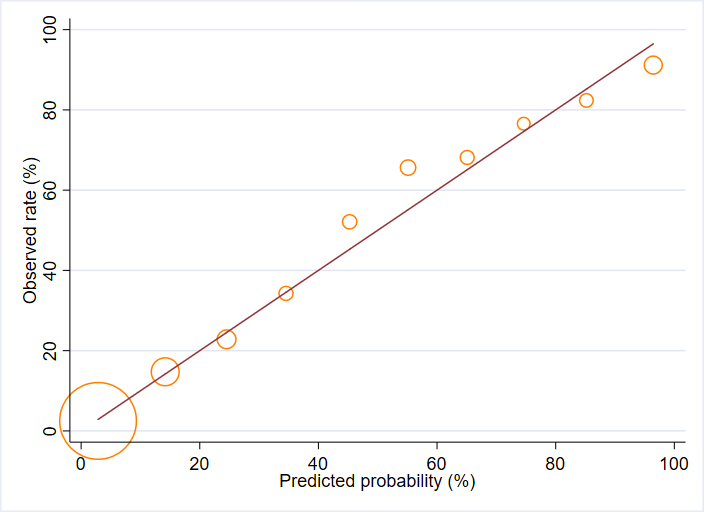
\includegraphics{atlas/Calib_bariatric.png} & 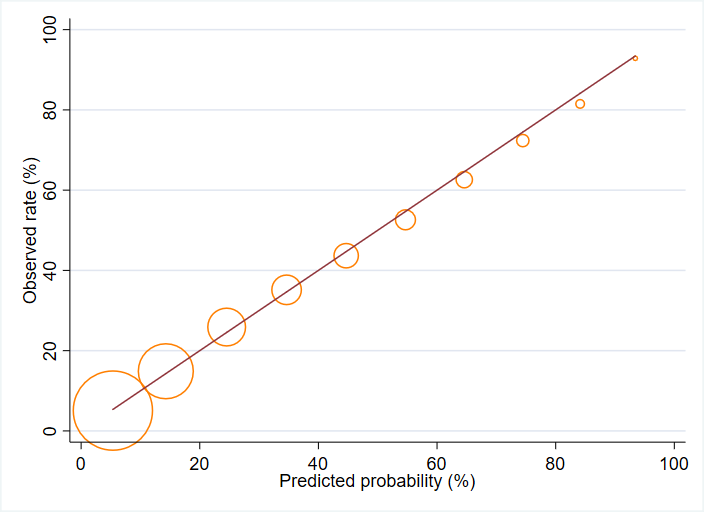
\includegraphics{atlas/Calib_cardio.png} & 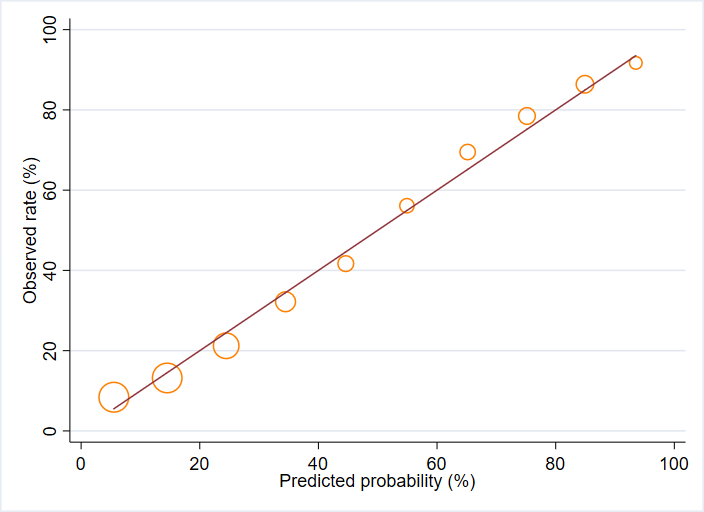
\includegraphics{atlas/Calib_KR.png} \\
Obstetric & Non-obstetric multiday & Non-obstetric sameday \\
\cmidrule(lr){1-1}\cmidrule(lr){2-2}\cmidrule(lr){3-3}
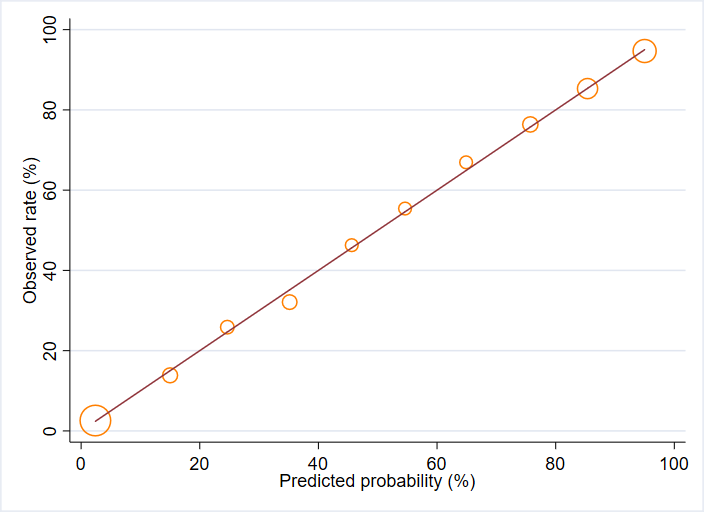
\includegraphics{atlas/Calib_obstetric.png} & 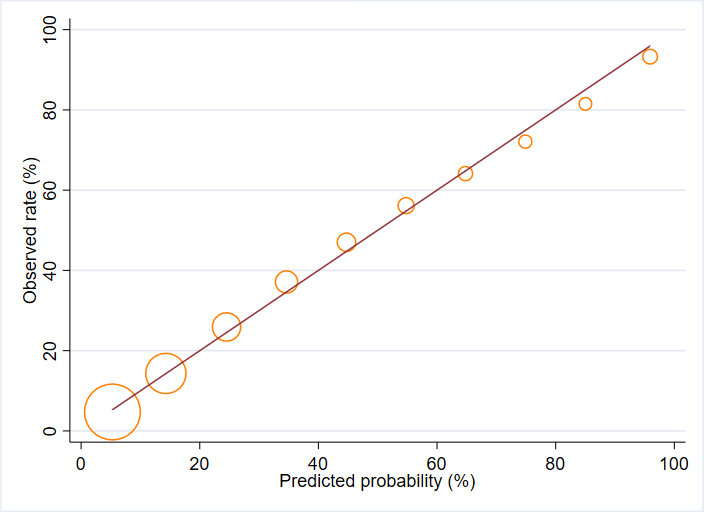
\includegraphics{atlas/Calib_non_obs_MD.png} & 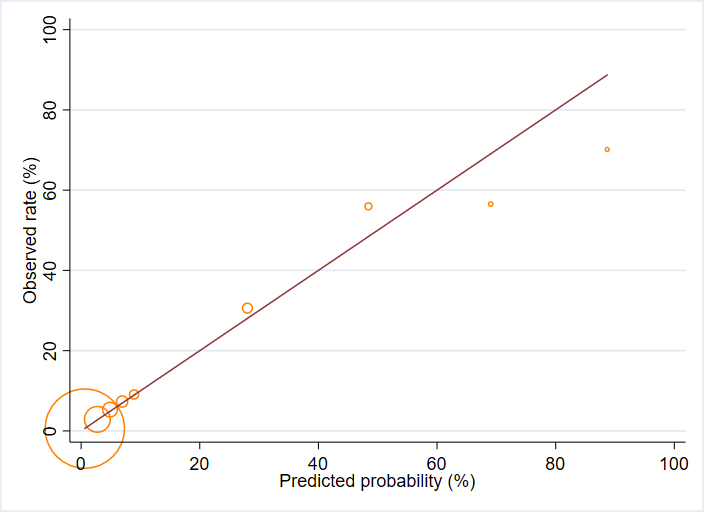
\includegraphics{atlas/Calib_non_obs_SD.png}
\end{tabularx}
\notewithsource{Calibration plot for the sameday non-obstetric subsample focuses on the first decile because almost all observations fell within that range.}%
{Grattan analysis of National Hospital Morbidity Dataset}
\end{figure*}

\begin{figure*}
\caption{All subsamples demonstrate satisfactory specificity and sensitivity}\label{fig:all-subsamples-satisfactory-specificity-sensitivity}
\units{Receiver Operator Characteristic curves by subsample}
\newcolumntype{C}{>{\centering\arraybackslash}X}
\setkeys{Gin}{width=0.33\textwidth}
\begin{tabularx}{\linewidth}{@{}C@{}C@{}C@{}}
Bariatric & Cardiology & Knee replacement \\
\cmidrule(lr){1-1}\cmidrule(lr){2-2}\cmidrule(lr){3-3}
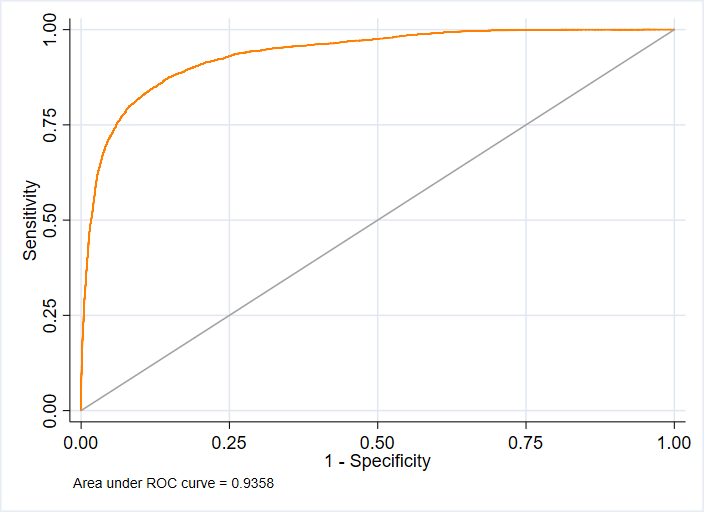
\includegraphics{atlas/ROC_bariatric.png} & 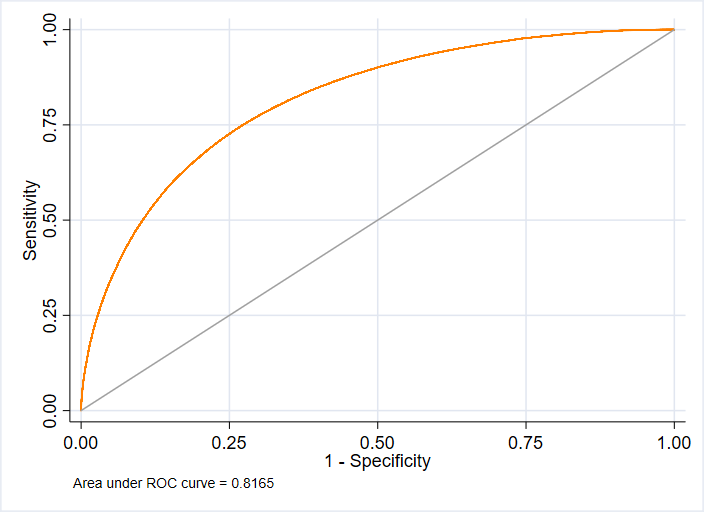
\includegraphics{atlas/ROC_cardio.png} & 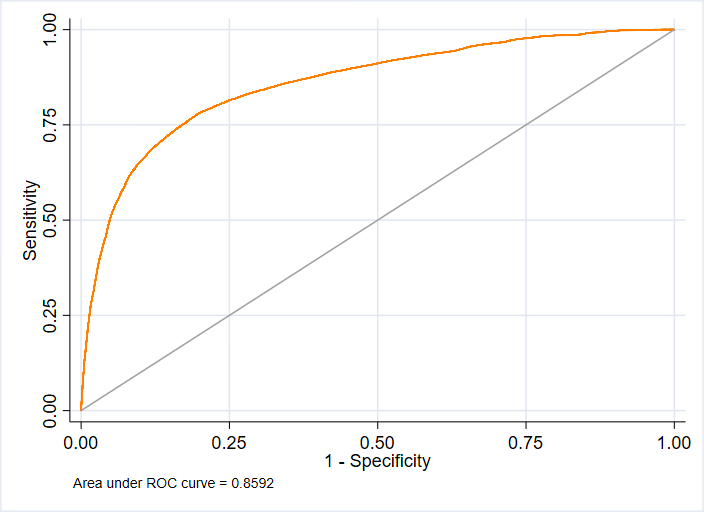
\includegraphics{atlas/ROC_KR.png} \\
Obstetric & Non-obstetric multiday & Non-obstetric sameday \\
\cmidrule(lr){1-1}\cmidrule(lr){2-2}\cmidrule(lr){3-3}
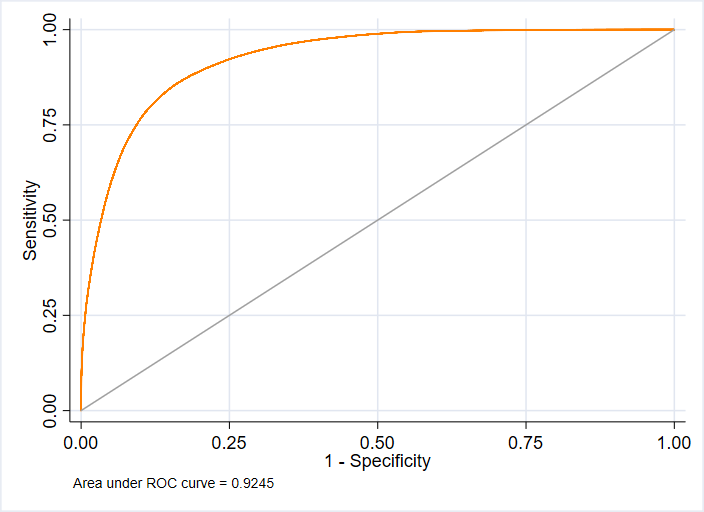
\includegraphics{atlas/ROC_obstetric.png} & 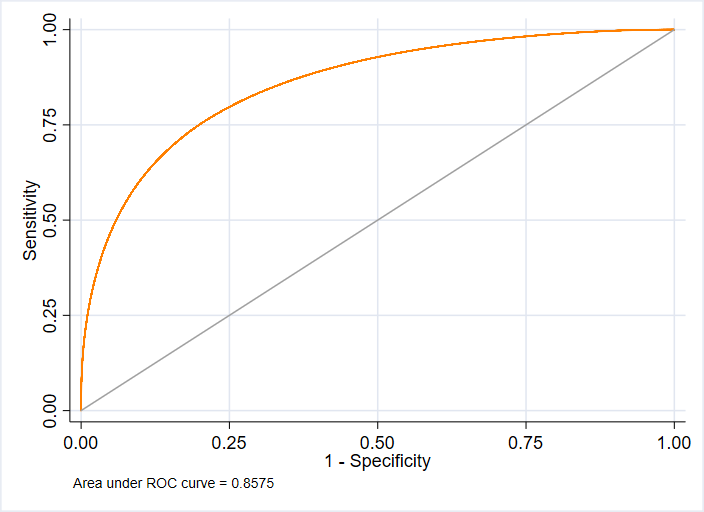
\includegraphics{atlas/ROC_non_obs_MD.png} & 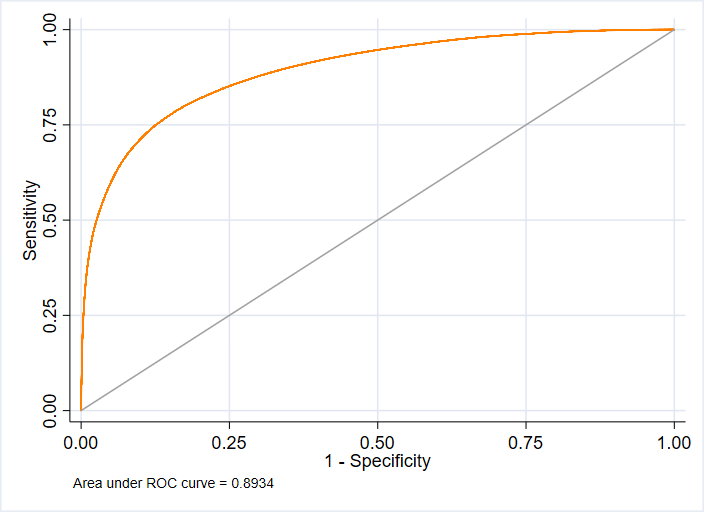
\includegraphics{atlas/ROC_non_obs_SD.png}
\end{tabularx}
\source{Grattan analysis of National Hospital Morbidity Dataset}
\end{figure*}

\subsection{Validity of model assumptions}\label{subsec:validity-of-model-assumptions}

In addition to assuring each model's in-sample fit, we have done our best to ensure the underlying assumptions of our model specification are valid.
The key assumptions are summarised in \Vref{box:model-assumptions}.
The assumptions pertaining to the random effects specification discussed in \Cref{sec:model-specification} are restated here as assumptions 3 and 5.

\begin{smallbox}{Model assumptions}{box:model-assumptions}

\begin{enumerate}[leftmargin=*]
\item[]\textbf{No multicollinearity: }

\item The independent variables are not collinear;

\textbf{No endogeneity: }

\item The residual term is not correlated with the independent variables;

\item The random effects terms are not correlated with the residual term;

\textbf{Distributional assumptions hold:}

\item The residual term is not over-dispersed;

\item The random effects estimates are approximately normally distributed.
\end{enumerate}
\end{smallbox}
\subsubsection{No multicollinearity}\label{subsubsec:no-multicollinearity}

We confirmed that our independent variables were not collinear by estimating the pairwise correlations between our independent variables.
Estimates of the correlations between patient-level covariates were all below 20 per cent.

Our two coding quality variables, coding depth and condition onset flag prevalence, were 50 per cent correlated.
While high, this correlation is still below the threshold of 80 per cent usually used to define collinearity.
This is not of great consequence because we do not aim to distinguish their contribution to patients' likelihood of having a complication recorded.
For the purpose of controlling for overall coding quality, the 50 per cent difference between these variables is sufficient to justify their inclusion.

\subsubsection{No endogeneity}\label{subsubsec:no-endogeneity}

As discussed in \Cref{subsec:the-inclusion-of-mundlak-means-in-the-risk-adjustment-model}, we protect against the most likely source of endogeneity: correlation between the random effects terms and covariates, proactively by including Mundlak means in our model specification.

As generally the case in outcomes research, there are other potential sources of endogeneity that could affect our model.
Length of stay is excluded because it's an intermediate outcome variable.
However, its exclusion could cause endogeneity via omitted variable bias.
Our data also contains little information about patients' health behaviours, religions and care preferences.
The exclusion of these types of risk factors could also some degree of endogeneity.
However, without a valid instrument, we can't test for or address these potential sources of endogeneity.
This is an inherent limitation of our model.

\subsubsection{Distributional assumptions hold}\label{subsubsec:distributional-assumptions-hold}

We assess whether our residual term is over-dispersed by comparing it to its assumed distribution.
With a sample size of \(N\) and with \(P\) parameters, the residuals of logit generalised linear models are assumed to be \(\chi^2\) distributed with \(N - P\) degrees of freedom.%
	\footcite{Collett-2003}
Consequently, a logit model can be said to be over-dispersed if the model's total error is greater than its degrees of freedom, and problematically so if total error exceeds the model's degrees of freedom by more than a factor of 5.%
	\footcite{CARRUTHERS_2008}
We estimate the dispersion of each of our models, \(\phi\), as follows:
\[\hat{\varphi}  = \frac{\text{Pearson \(\chi^{2}\) statistic}}{N - P} = \frac{\sum_{d = 1}^{10}\frac{\left( O_{d} - E_{d} \right)^{2}}{E_{d}}}{N - P}\]

\Vref{tbl:estimated-dispersion-by-model} presents our estimated dispersion parameters by subsample.
It shows that all of the models exceed the assumed rate of dispersion of one, but not by much except for the non-obstetric multiday sample.
Such low dispersion is a positive indication of models' fit, as over-dispersion is very much the norm in practice.
It is likely to be attributable to the realistic way our multilevel model structure accounts for independence between outcomes.%
	\footcite{Stata-multilevel-modelling}

\begin{table}
\caption{Estimated dispersion by model}\label{tbl:estimated-dispersion-by-model}
\begin{tabularx}{\linewidth}{l>{\raggedleft}RR}
\toprule
& \textbf{Estimated dispersion parameter} & \textbf{Is this model over-dispersed?}\tabularnewline
\midrule
Non-obstetric MD & 14.22 & Yes\tabularnewline
Non-obstetric SD & 1.26 & No\tabularnewline
Obstetric & 1.22 & No\tabularnewline
Cardiology & 1.01 & No\tabularnewline
Knee replacement & 1.29 & No\tabularnewline
Bariatric & 2.10 & No\tabularnewline
\bottomrule
\end{tabularx}
\vspace{1\baselineskip}
\null
\end{table}

The over-dispersion of our model on the non-obstetric multiday subsample is likely to be attributable to the substantial heterogeneity of the patients included in this sample, which limits the accuracy with which it's possible for us to adjust for patients' risk profiles.
We draw this conclusion because other common causes of over-dispersion in logit models, such as an incorrect choice of link function, influential outliers or an exceedingly rare dependent variable, are more true of the subsamples which do not exhibit this shortcoming.%
	\footcite{Collett-2003}

The over-dispersion may bias the standard error estimates of this model, so we refrain from drawing conclusions from this sample that are not also supported in our case studies.
However, we note that this model still performed favourably on measures of goodness of fit.

\Vref{fig:hospital-perf-approximately-normal-case-studies,fig:hospital-perf-approximately-normal} demonstrate that our additional assumption regarding the normality of the random effects terms is also reasonably well supported.
These estimates of the distribution of hospital performance by subsample are not perfectly normal, but we note model estimates have been found to be robust to modest misspecification of random effects' distributions.%
	\footcite{Neuhaus_2011}


\doublecolumnfigure{
\caption{Hospital performance is approximately normally distributed across our case studies}\label{fig:hospital-perf-approximately-normal-case-studies}
\units{Kernel densities of hospital random effects terms by subsample}
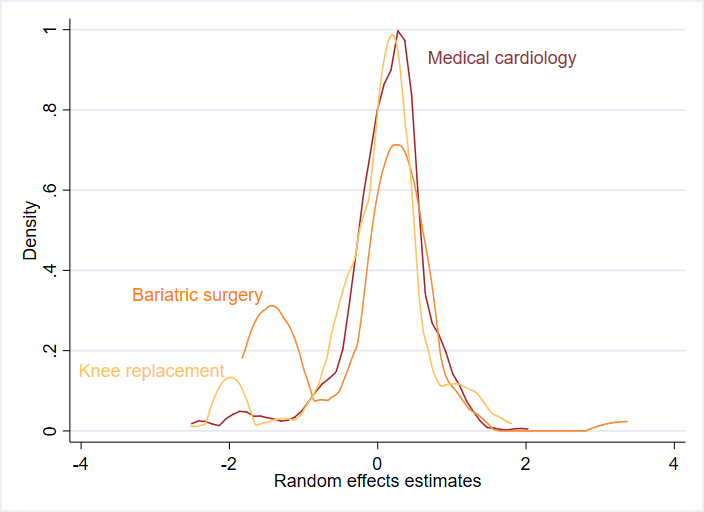
\includegraphics{atlas/Case_studies_kernel_density.png}
\noteswithsource{Densities have been estimated using an Epanechnikov kernel with bandwidths ranging from 0.1 to 0.2 on the raw random effects terms, depending on the series' volatility.}%
{Grattan analysis of the 2012-15 National Hospital Morbidity dataset}
}{
\caption{Hospital performance is approximately normally distributed across our full sample}\label{fig:hospital-perf-approximately-normal}
\units{Kernel densities of hospital random effects terms by subsample}
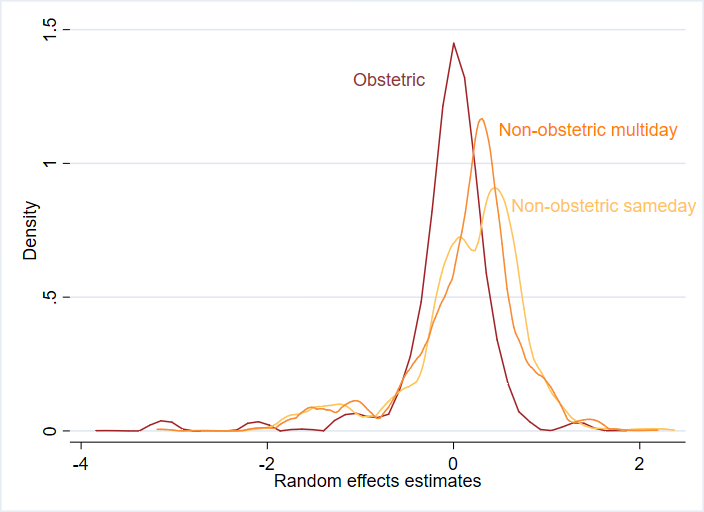
\includegraphics{atlas/Full_sample_kernel_density.png}
\noteswithsource{Densities have been estimated using an Epanechnikov kernel with bandwidths ranging from 0.1 to 0.2 on the raw random effects terms, depending on the series' volatility.}%
{Grattan analysis of the 2012-15 National Hospital Morbidity dataset}
}

\begin{smallbox}{Conclusions of the hypothesis test}{box:procedural-complications-increase-length-of-stay}
\null\vspace{0.5\baselineskip}

\captionof{table}{Procedural complications increase length of stay}\label{tbl:procedural-complications-increase-length-of-stay}
\begin{tabularx}{\linewidth}{lRR}
\toprule
& \textbf{Marginal effect} & \textbf{P-value}\tabularnewline
\midrule
Non-obstetric multiday & 4.93 & 0.000\tabularnewline
Multiday knee replacement & 2.10 & 0.000\tabularnewline
Multiday bariatric surgery & 4.34 & 0.000\tabularnewline
\bottomrule
\end{tabularx}
\vspace{0.5\baselineskip}

These hypothesis tests relating to the marginal effect of procedural complications on length of stay are derived from models on each subsample that are specified as follows:
\[\text{length of stay} =  \beta_{0} + \beta_{1}\,\mathrm{MCHADx1} + \beta_{2}\,\text{Age} + \beta_{3}\,\text{Sex} + \varepsilon\]

The marginal effect of incurring at least one procedural complication is given by \(\beta_{1}\) in the model specification.

Reported p-values relate to the hypothesis test of whether \(H_{0}:\beta_{1} = 0\) or \(H_{1}:\beta_{1} \neq 0\).
\end{smallbox}

\section{Other supporting analysis}\label{sec:other-supporting-analysis}

Not all of the analysis contained in \textit{\myTitle} is based on the outcomes research models.
In this section, we describe the methodologies for supporting pieces of analysis.

\subsection{Complications and length of stay}\label{subsec:complications-and-length-of-stay}

One metric with which to measure the impact of a complication on patients' wellbeing is number of extra days in hospital that is associated with it, on average.
However, the impact of complications on length of stay is difficult to quantify because length of stay generally also affects the likelihood of most complications occurring.%

Conscious of this obstacle, we chose to focus our inquiry into complications' impact on length of stay on post-procedural complications.
Post-procedural complications are not endogenous with length of stay in the same way as adverse drug events because the risk of these complications increases with the number of procedures a patient undergoes, rather than the days in hospital.
This makes patients who undergo a single, standardised operation, like knee replacements patients, an appropriate focus for this type of analysis.

\Figure{1.2} of \textit{\myTitle} presents the differences in average length of stay for patients who do and do not experience procedural complications, by sample of admissions. \Cref{tbl:procedural-complications-increase-length-of-stay} in \Vref{box:procedural-complications-increase-length-of-stay} presents the conclusions of our formal hypothesis tests that length of stay differs among patients on the basis of whether they experienced a post-procedural complication, for each sample.



\subsection{Hospital performance aggregated to minor CHADx+}\label{subsec:hospital-performance-aggregated-to-minor-chadx}

Making up the Classification of Hospital Acquired Diagnoses are 17 major classes of complications, and 159 complications. \textit{\myTitle} recommends that risk-adjusted data on each complication and each major CHADx+ class is provided to hospitals, as well as risk adjusted data on their overall prevalence of any complication.

In Chapter~4 of \textit{\myTitle}, we provide an example of how each individual hospital's data could be reported to them as a risk-adjusted heat map.
The first column of the chart is colour coded by the hospital's quintile of performance by each major CHADx+ class, and the subsequent columns indicate the hospital's quintile of performance in each of the specific complications that make up each major CHADx+ class.
This analysis was completed on non-obstetric multiday admissions.

To obtain these risk-adjusted estimates of hospitals' relative performance on specific complications, we estimate additional outcomes research models: one for each complication and for each of the 17 major classes of complications.

Without sufficient time or computing resources to fit each of these models using a random effects, or even fixed effects, model specification, we used a pooled effects model specification for this segment of the analysis.
This is similar to the approach employed in IHPA's risk adjustment model for Hospital Acquired Complications.%
	\footcite{IHPA-2017-Risk-adj-model-tech-specs}

To expedite this exercise, we use the patient risk term previously estimated in relation to the prevalence of any complication.
We combine this risk factor with the hospital-level risk factors in a logit risk adjustment model:
\[\log\left( \frac{p_{i}}{1 - p_{i}} \right) = \beta_{1}X_{i,1} + \ldots + \beta_{K}X_{i,K} + \varepsilon_{i}\]

Where:

\begin{description}
\item[\(p_{i}\)] is the probability that patient \(i\) experiences a given complication;
\item[\(X_{i,1},\dots,X_{i,K}\)] are the risk factors included in the model, evaluated relative to patient \(i\);
\item[]
  And the residual term is normally distributed and homoscedastic: \(\varepsilon_{i} \sim N(0,\sigma^{2})\).
\end{description}

From this model, we predict the expected log-odds ratio, \(r_{i}\), of each complication for the average patient of each hospital.
We convert these to the probability that the average patient from each hospital, \({h}\), experiences a complication using the transformation:
\[{\hat{p}}_{{h}} = \frac{\exp({\hat{r}}_{{h}})}{1 + \exp( {\hat{r}}_{h} )}\]

The probability that a hospital's average patient experiences a given complication can be interpreted as the expected rate of that complication for that hospital.
Accordingly, we compute the observed to expected ratio of complications used to measure hospital performance from pooled specifications of outcomes research models using \(\hat{p_{i}}\):
\[\text{Hospital performance}_{c,h} = \frac{\sum_{i \in h}^{}{\mathrm{CHADx}_{c}}/n_{h}}{{\hat{p}}_{h}} = \frac{\text{Observed\ rate}_{c,h}}{\text{Expected\ rate}_{c,h}}\]

Where:

\begin{itemize}
\item[\(c\)] indicates the complication of interest
\item[\(h\)] identifies any particular hospital
\item[\(n_{h}\)] is the number of admissions within hospital \(h\)
\end{itemize}

Using this methodology, risk adjusted estimates of hospitals' performance in each complication and major class of complications were obtained.
The exemplar for our proposed reporting scheme was then colour coded on the basis of which quintile of performance hospital 1 was classified in for each complication and major CHADx+ class.

\section{Stability analysis}\label{sec:stability-analysis}

In \Cref{subsec:accounting-for-differences-in-coding-quality}, we discussed the importance of ensuring performance metrics are representative of hospitals' usual performance, rather than being prone to mean reversion.
We have taken several precautions in our analysis to ensure this is the case.

However, \textit{\myTitle} also recommends that hospital performance is reported on regularly and granularly.
This raises the more general question of which indicators are sufficiently stable to be useful measures of hospitals' performances, and under what circumstances.

There are four factors that affect the stability of a performance metric.
Fundamentally, performance metrics are more stable when random chance plays a smaller role in determining its incidence, and when the underlying event is more common.%
\footnote{That is, stability increases alongside a metric's coefficient of dispersion.}
Metrics are also more stable when they're measured across bigger institutions, or over longer periods of time.
Whether a metric is stable \emph{enough} depends on the level of detail and reliability required of the estimate.

For the purpose of exploring these relationships, we investigate whether particular performance metrics are stable enough to reliably identify a hospital's decile of performance.%
\footnote{This is an arbitrary threshold and could readily be tailored to a particular policy objective.}
To do this, we first calculate the average amount that a hospital's metric varies across consecutive periods, and then scale it by the average width of that metric's deciles:
\begin{align*}
\text{Stability}_{M} &= \frac{1}{H(T-1)}\sum_{h = 1}^{H} \left(\sum_{t = 2}^T(M_{h,t} - M_{h,t - 1}) \right)\\
\text{Average\ decile\ width}_{M} &= \frac{1}{9}\sum_{d = 10}^{100}{(Q_{M, d} - Q_{M, d - 1})}\\
\text{Scaled\ stability}_{M} &= \frac{\text{Stability}_{M}}{\text{Average\ decile\ width}_{M}}
\end{align*}

Where:

\begin{itemize}
\item[\(M\)] is any given metric, which takes the value \(M_{h,t}\) for hospital \(h\) in period \(t\);
\item[\(Q_{M,d}\)] refers to the \(d\)\textsuperscript{th} quantile of metric M
\item[\(h\)] is any of the \(H\) hospitals
\item[\(t\)] is any of the \(T\) time periods
\item[\(d\)] refers to any number in the series: 10, 20, \dots{}, 80, 90, 100.
\end{itemize}

We identify the minimum sample size for which \(\text{scaled stability}_{M} \leq 1\) by splitting our data into seven categories by hospital size, estimating \(\text{scaled stability}_{M}\) for each of these subsamples and fitting a line with the following functional form fit to these seven data points:%
  \footnote{Fewer than seven data points were used in some cases to make the fitted lines less sensitive to outliers.}

\[\text{Scaled stability}_{M} = b*\ln\left( \text{hospital\ size} \right) + c\]

This simple model specification explains about on average roughly 80 per cent of variation in the scaled stability of each of the indicators assessed.%
\footnote{Assessing three variables (CHADx+, MCHADx5, HACs) across four time periods (monthly, quarterly, six-monthly, annually), we estimated this relationship across 12 subsamples.}
We infer the minimum hospital size for which we can expect a metric's stability to be less than or equal to with the width of a decile as follows:

\[(\text{Hospital size} \mid \text{Scaled stability}_{M} = 1) = \exp\left( \frac{1 - \hat{c}}{\hat{b}} \right)\]

Where \(b\) and \(c\) are the parameters of the model, and are estimated from the data to take the values \(\hat{b}\) and \(\hat{c}\).

\begin{figure}
\caption{Some indicators are much more stable than others}\label{fig:some-indicators-are-much-more-stable-than-others}
\units{Minimum hospital size required to be able to reliably identify the decile of a hospital's performance}
\includegraphics[page=35]{atlas/comps_charts.pdf}
\noteswithsource{We consider an indicator to be able to reliably identify the decile of a hospital's performance over a particular sample if the average change in hospitals' rates between periods is less than the average range of a performance decile.}{Grattan analysis of the 2012-15 National Hospital Morbidity Dataset}
\end{figure}

We find that overall complication rates are actually quite stable within hospitals.
For example, a single performance decile spans a four per cent range of complication rates, on average, and complication rates at hospitals with at least 600 admissions a year tend to vary across years by less than this amount.%
\footnote{Of course, extreme deciles are wider and moderate performance deciles are narrower than this average range.}
This implies that, when hospitals are compared on the basis of their overall complication rates, it's likely that they'll be ranked in the same performance decile in each consecutive year -- even if they are a relatively small hospital.%
\footnote{More precisely, they're likely to be \emph{within a decile} of their previous position, which includes the scenario where a hospital moves from the upper bounds of one decile to the lower bounds of the above decile.}

\Cref{fig:some-indicators-are-much-more-stable-than-others} illustrates how this stability changes when performance is measured over a shorter period, or when only a particular group of complications are considered.
As expected, performance metrics are less stable when measured over shorter periods of time.
Still, rates of all types of complication looked at here are stable enough to identify a hospital's precise decile of performance for hospitals with 3000 or more admissions per year.

Importantly, we also observe that HACs and cardiology complications are substantially less stable measures than the incidence of complications overall.
This is in line with our expectations: affecting approximately 2 per cent of admissions, these subsets of complication affect only a fifth of patients that experience any complication.
Consequently, their incidence will be more volatile.

\Cref{fig:some-indicators-are-much-more-stable-than-others} usefully clarifies two characteristics of this relationship.
Firstly, which outcome is measured has a greater impact on the stability of the outcome metric than the length of time over which it is measured.
Secondly, the prevalence of a particular event affects -- but does not determine -- a metric's stability.
We note that HACs and cardiology complications are equally prevalent, yet hospitals' rates of cardiology complications are more stable.%
\footnote{This does not imply one measure is necessarily superior, just that the stability of particular metrics cannot be inferred from their prevalence.}



In total, this analysis provides useful assurance that there is enough information amongst the noise to distinguish hospitals' performances with reasonable precision, even over short time periods or using relatively rare events.%
	\footnote{We emphasise that this analysis uses raw prevalence rates.
	Extending this analysis to risk adjusted complication rates would be a worthwhile endeavour.}
While the stability of metrics is not self-evident, it is readily assessable -- especially relative to decision criteria.
Like analysis should be repeated to determine whether particular metrics are stable \emph{enough} for a given policy objective, for the hospital size and measurement window of interest.


\chapter{Additional details regarding proof-of-concept app}\label{chap:app-disclaimer}
In \emph{All complications should count} we refer to an app that Grattan Institute has developed as a proof-of-concept. The app presents the average complication rates for elective surgical procedures by age, sex, specialty and the length of the patient's stay, using admissions data from 2012 to 2015. Results produced by the app should be taken as indicative only.

No personal information is disclosed by this app.
Only subgroups with more than 20 admissions in each of the years were used, 
only counts and averages are used for each subgroup, and
the original data was perturbed before the tables were prepared and uploaded.

Grattan Institute recognizes the significant foundational work undertaken by the Health System Planning and Investment Branch, NSW Ministry of Health, which has informed the development of this work.


\printbibliography
\end{document}
